% Created 2021-02-15 Mon 18:18
% Intended LaTeX compiler: xelatex
\documentclass[letterspacing]{tufte-book}
\usepackage{graphicx}
\usepackage{longtable}
\usepackage{wrapfig}
\usepackage{rotating}
\usepackage[normalem]{ulem}
\usepackage{amsmath}
\usepackage{textcomp}
\usepackage{amssymb}
\usepackage{capt-of}
\usepackage{hyperref}
\usepackage{ucs}
\usepackage{xeCJK}
\setCJKmainfont{STXihei}
\setkeys{Gin}{width=\linewidth,totalheight=\textheight,keepaspectratio}
\usepackage{booktabs} % book-quality tables
\usepackage{units}    % non-stacked fractions and better unit spacing
\usepackage{multicol} % multiple column layout facilities
\usepackage{fancyvrb} % extended verbatim environments
\fvset{fontsize=\normalsize}% default font size for fancy-verbatim environments
\usepackage{listings}
\lstset{basicstyle=\ttfamily\normalsize,breaklines=false,frame=l}
\setcounter{secnumdepth}{3}
\author{欧阳继超}
\date{\textit{<2017-02-10 Fri>}}
\title{Grokking Monad\\\medskip
\large 函数式装逼手册}
\hypersetup{
 pdfauthor={欧阳继超},
 pdftitle={Grokking Monad},
 pdfkeywords={},
 pdfsubject={},
 pdfcreator={Emacs 27.1 (Org mode 9.3)}, 
 pdflang={English}}
\begin{document}

\maketitle
\tableofcontents

\newpage
\begin{fullwidth}
~\vfill
\thispagestyle{empty}
\setlength{\parindent}{0pt}
\setlength{\parskip}{\baselineskip}
Copyright \copyright\ 2015-\the\year\ Jichao Ouyang

Printable is generated from free softwares: GNU Emacs, orgmode, Tex, Graphivz DOT...
\par\url{github.com/jcouyang/grokking-monad}

\par\textit{First printing, 2020}
\end{fullwidth}

\chapter*{前言}
本书的主要目的是为了解释 \textbf{为什么需要*, *如何理解} 以及 \textbf{如何使用} Monad,
分为三大个部分,猫论/Catergory Theory,食用猫呢/Practical Monads和搞基猫呢/Advanced Monads。\footnote{什么?你不喜欢谐音梗?我也不喜欢,可是,这也不是讲脱口秀的书啊。 \sout{再说你也就花了六美元,十分适合这种廉价梗}}

\begin{quote}
\textbf{猫论/Catergory Theory} 是理论基础,解释单子由何而来,若是 \sout{不想装逼装得有理有据} 觉得太无聊其实可跳过,比较适合好奇心大的猫。

\textbf{食用猫呢/Practical Monads} 提供很多日常会遇到的单子供大家食用。

\textbf{搞基猫呢/Advanced Monads} 适合谁你自然懂得。
\end{quote}

其中所有例子都有双语 \sout{中文和英语} \emph{Haskell} 和 \emph{Scala} 解释,双语例子都成对出现,先 Haskell 后 Scala。

至于为什么选择这两种语言?其实代表两大派系,一个ML系一个Java/C++系,若是看不懂 Haskell,Scala 可能
会更好懂些。

当掌握了这种思维方式,不局限于 Haskell 或者 Scala,其实可以扩展到任何语言的编程中,即使是没有类型系统的语言,JS,说你呢,不要看人家PHP。

\begin{quote}
那么,为啥要花钱买一本不是正规出版社的书?
\end{quote}

许多年前,当我还是年少 \sout{有为} 无知的时候,有个很正规的出版社叫我写过一本书\footnote{\url{https://book.douban.com/subject/26883736/}}。

当我听说写书是按字数给钱的时候,我的程序员世界观崩塌了那么一会。
什么 DRY\footnote{不要重复(Don't Repeat Yourself) \url{https://en.wikipedia.org/wiki/Don\%27t\_repeat\_yourself}},什么 YAGNI\footnote{你可能不会需要的(You Aren't Gonna Need It) \url{https://en.wikipedia.org/wiki/You\_aren\%27t\_gonna\_need\_it}},我统统都需要,而且能重复说的概念绝对不能一次说清楚了。

那段时光里 Emacs 那熟练的快捷键 \texttt{Ctrl y} 简直就是我的人民币印钞机。

于是我东拼西凑,从我的博客抄了好多字。结果豆瓣才6.6分,居然只有几个人说我是抄的, \sout{真是的,读书人,怎么能说抄呢?} 显然读者都不怎么看我的博客。

再说了, \sout{我抄你家书了吗?} 其实书上可比我的博客精致多了,看,我还加了好多萌萌的插画呢。字不算钱,画也多少算点吧。而且,老子写博客的时间不要钱吗?

呵呵,确实不要。

显然第一版还滞销,出版社也再没联系我第二版的版税💰的事情。就这么投入一年的时间加工精美博客以获得利润的完美赚钱计划,结果还不如我打工一天赚的钱多。

不过不叫确实好怪我,目标读者是前端,内容显然过于 \sout{超前} 乏味了些。但是卖不掉我还真是严重怀疑是因为出版社设计的书皮太难看。

你看看那橘色的封面,跟 Emmet\footnote{Emmet Brickowski:乐高大电影里的一名普通建筑工人。咦,普通工人怎么有wiki?我都没有 \url{https://thelegomovie.fandom.com/wiki/Emmet\_Brickowski}} 的工服一个颜色,你很难想象这不是一本建筑工程师的书。
我要是在图书馆看见这本书,我都怀疑自己走错了到了建筑装潢区,对啊我本来是来借啥书来着?我在哪?我是谁?

你看,这种水平的前言,出版社肯定不乐意要让我改,但是我乐意啊,啊哈哈哈哈。

哦,对,还没说这本书是啥情况呢。其实这本书,它…也是从我的同名博客\footnote{\url{https://blog.oyanglul.us/grokking-monad/part1}}抄的…

但其\ldots{}实我还是有加入更多的内容\footnote{比如,你看,博客里就没有这篇前言。},更重要的是这个超有设计感的封面。

你想想,六美元\footnote{啊,那为啥是以美元为单位?那是因为 Gumroad 是按美元给我结算,这样我可以挑选合适的的时候换算成澳元或者人民币花,啊哈哈哈。}可以买两瓶可乐,六美元能买一本儿童涂色书,六美元能买二分之一顿饭。
你少喝两瓶可乐,让你娃少涂一本涂色书,你少吃半顿饭,买了这本书,把里面的词汇都背下来,在同事领导面前时不时冒出一两个来装逼,升值加薪不是梦。

或者,打印出来但千万不要装订,抱在怀里从女神男神面前走过时不小心撞一下顺势往天上这么一撒,女神男神在慌乱中一起帮你捡地上散落的书时,肯定会惊叹:哇,这人好厉害居然知道Monad是什么?
再加上刚才撞一下引起的心跳加速,对你的好感油然而生。

只是少喝两瓶可乐,少涂一本涂色书,少吃半顿饭省下来的六美元\footnote{你看我这写上本书落下的 \texttt{Ctrl y} 毛病。},就能提前助你走上人生巅峰的感觉,难道不六吗?


\part{猫论/Catergory Theory}
\label{sec:orga332599}

\begin{center}
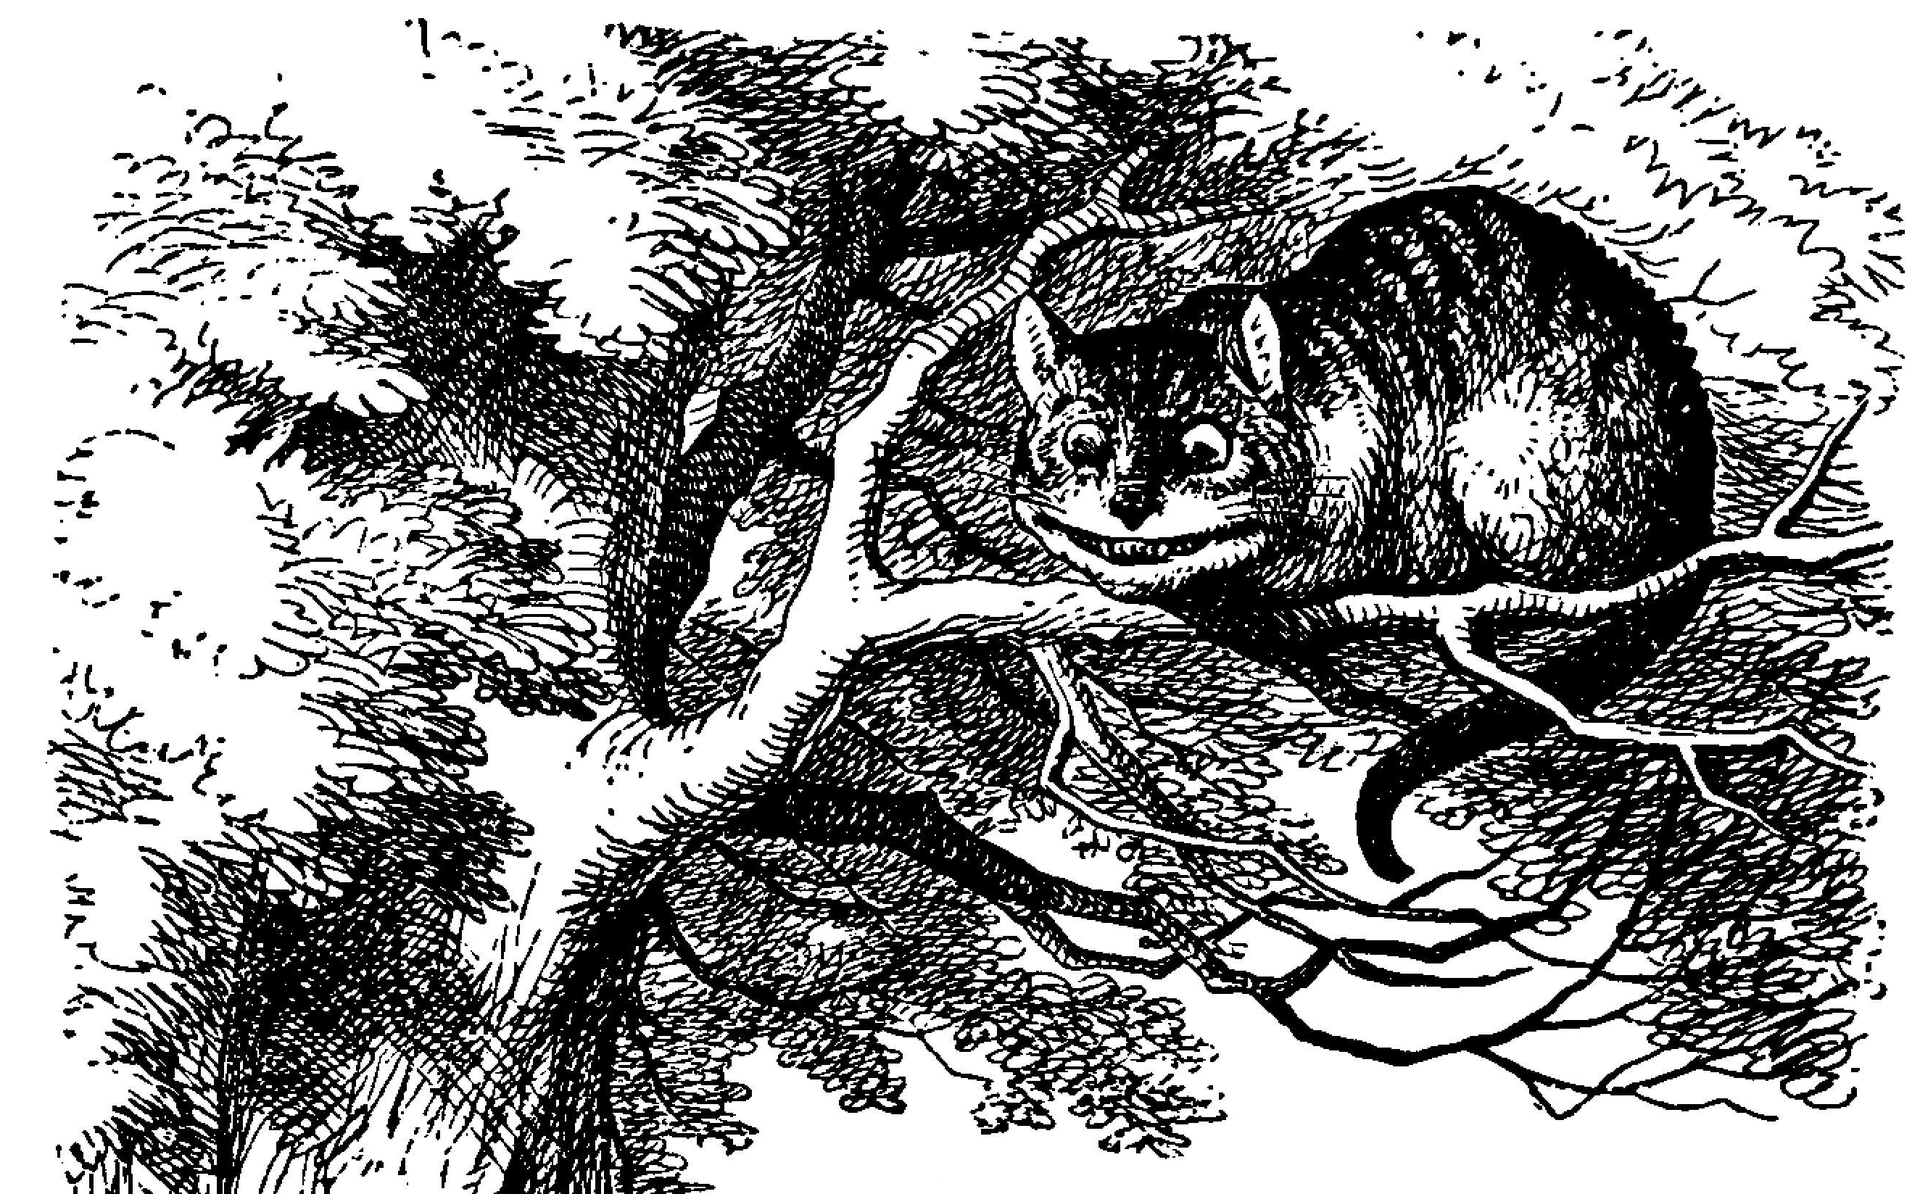
\includegraphics[width=.9\linewidth]{./images/Cheshire_Cat.png}
\end{center} \footnote{\url{https://en.wikipedia.org/wiki/Cheshire\_Cat}}

\begin{quote}
`But I don’t want to go among mad people,’ Alice remarked.

`Oh, you can’t help that,’ said the Cat: `we’re all mad here. I’m mad. You’re mad.’

`How do you know I’m mad?’ said Alice.
`You must be,’ said the Cat, `or you wouldn’t have come here.’

Alice didn’t think that proved it at all; however, she went on `And how do you know that you’re mad?’

-- Alice's Adventures in Wonderland
\end{quote}

\begin{quote}
单子/Monad是什么? 你也不懂, 我也不懂, 我们都不懂.

话说, 我又怎么知道你不懂呢?

当然不懂, 不然, 你怎么会来到这里?

我又是怎么知道自己不懂呢?

因为,我知道懂的人是什么样子. 显然, 我不是.

因为,懂的人一定知道猫论/Category Theory.
\end{quote}

这一部分主要是纯理论,这里面有很多很装的单词,比如 \emph{单子/Monad/,它们都是 /斜体}
,就算一遍没看懂\footnote{可以继续看第二部分,看完概念是如何在现实中实现的,再回来看一遍,会感觉好很多。},把这些词背下来也足够装好长一阵子逼了。

这里还有很多代码, 它们都成对出现, 通常第一段是 Haskell, 第二段是 Scala 3.\footnote{为什么用两种语言呢?第一: \sout{这样代码量会翻倍,可以凑篇幅字数。} 这样大家会熟悉多种语言对同一概念的诠释,从而举一反三。
第二:读者受众会大一点,因为毕竟Haskell的表述比较简洁,有可能很容易理解,但是跟主流语言的表达方式大为不同,也有可能很难适应,加上表达方式更为具体的 Scala,便于加深理解。}

\chapter{范畴/Category}
\label{sec:orge141111}
\index{Catergory}
\index{范畴}

对于计算机科学的学生,范畴并不是一个新的概念,在本科大纲里,大家都应该学过 \emph{离散数学(Discrete Mathematics)} ,其中会讲很多 \emph{集合论(Set Theory)} 图论,抽象代数的东西。
现在回头看看,其实也就是集合论和抽象代数的内容。

所以下面的概念都点到为止,只为解释写成代码会长什么样。

一个 \emph{范畴/Category} 包含两个玩意:
\begin{itemize}
\item 东西 \texttt{O} (Object)
\item 两个东西的关系,箭头 \texttt{\textasciitilde{}>} ( \emph{态射/Morphism} )
\end{itemize}

还必须带上一些属性:
\begin{itemize}
\item 一定有一个叫 id 的箭头,也叫做 1
\item 箭头可以 \emph{组合} compose/
\end{itemize}

恩, 就是这么简单!

\begin{figure}[htbp]
\centering
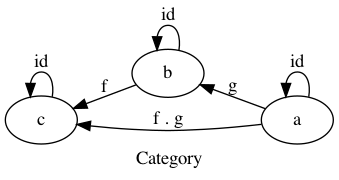
\includegraphics[width=.9\linewidth]{images/category.png}
\caption{有东西 a, b, c 和箭头 f, g 的 Category,其中 f . g 表示 compose f 和 g}
\end{figure}


\begin{quote}
注意到为什么我会箭头从右往左,接着看代码, 你会发现这个方向跟 compose 的方向刚好一致!
\end{quote}

这些玩意对应到 Haskell 的 Typeclass 大致就是这样:

\lstset{language=haskell,label= ,caption={Category definition in Haskell},captionpos=b,numbers=none}
\begin{lstlisting}
class Category (c :: * -> * -> *) where
  id :: c a a
  (.) :: c y z -> c x y -> c x z
\end{lstlisting}

如果这是你第一次见到 Haskell 代码,没有关系,语法真的很简单:
\begin{itemize}
\item \texttt{class} 定义了一个 TypeClass, \texttt{Category} 是这个 TypeClass 的名字
\item Type class 类似于定义类型的规范,规范为 \texttt{where} 后面那一坨
\item 类型规范的对象是参数 \texttt{(c:: * -> * -> *)} , \texttt{::} 后面是c的类型
\item c 是 \emph{higher kind} \texttt{* -> *} ,跟higher order function的定义差不多,它是接收类型,构造新类型的类型。这里的 c 接收一个类型,再接收一个类型,就可以返回个类型。
\end{itemize}
\index{Kind}
\begin{itemize}
\item \texttt{id:: c a a} 表示 c 范畴上的 a 到 a 的箭头
\item \texttt{.} 的意思 c 范畴上,如果喂一个 y 到 z 的箭头,再喂一个 x 到 y 的箭头,那么就返回 x 到 z 的箭头。
\end{itemize}

而 Scala 可以用 trait 来表示这个 typeclass:
\lstset{language=scala,label= ,caption={Category definition in Scala},captionpos=b,numbers=none}
\begin{lstlisting}
trait Category[C[_, _]] {
  def id[A]: C[A, A]
  def <<<(a: C[Y, Z], b: C[X, Y]): C[X, Z] 
}
\end{lstlisting}

如果这是你第一次见到 Scala 代码,没关系,从Haskell可以飞快的切换过来:
\begin{itemize}
\item \texttt{class} -> \texttt{trait}
\item[{=c}] * -> * -> *= -> \texttt{C[\_, \_]}
\item \texttt{::} -> \texttt{:}
\item 函数名前加 \texttt{def}
\end{itemize}

另外 compose 在 haskell 中直接是句号 \texttt{.}

scala 中用习惯用 \texttt{<<<} 或者 \texttt{compose}

总之,我们来用文字再读一遍上面这些代码就了然了.

范畴 C 其实就包含:
\begin{enumerate}
\item 返回 A 对象到 A 对象的 id 箭头
\item 可以组合 Y 对象到 Z 对象 和 X 对象到 Y 对象的箭头 compose
\end{enumerate}

简单吧?还没有高数抽象呢。

\section{\emph{Hask}}
\label{sec:org2bda925}
Haskell 类型系统范畴叫做 Hask。
\index{Hask}

在 Hask 范畴上:

\begin{itemize}
\item 东西就是类型
\item 箭头是类型的变换,即 \texttt{->}
\item id 就是 id 函数的类型 \texttt{a -> a}
\item compose 当然就是函数组合的类型
\end{itemize}

\lstset{language=haskell,label= ,caption= ,captionpos=b,numbers=none}
\begin{lstlisting}
type Hask = (->)
instance Category (Hask:: * -> * -> *) where
  id a = a
  (f . g) x = f (g x)
\end{lstlisting}

我们看见新的关键字 \texttt{instance} ,这表示 Hask 是 Type class Category 的实例类型,也就是说对任意Hask类型, 那么就能找到它的 id 和 compose

\lstset{language=scala,label= ,caption= ,captionpos=b,numbers=none}
\begin{lstlisting}
given Category[=>[_, _]] {
  def id[A]: A => A = identity[A]
  def <<<[X, Y, Z](a: Y => Z, b: X => Y) = a compose b
}
\end{lstlisting}

Scala 中, 只需要 new 这个 trait 就可以实现这个 typeclass

其中: identity \texttt{Hask a a} 就是
\lstset{language=haskell,label= ,caption= ,captionpos=b,numbers=none}
\begin{lstlisting}
(->) a a -- or
a -> a -- 因为 -> 是中缀构造器
\end{lstlisting}

\lstset{language=scala,label= ,caption= ,captionpos=b,numbers=none}
\begin{lstlisting}
A => A
\end{lstlisting}
\section{\emph{Duel}}
\label{sec:org5481e33}
\index{Duel}
每个 Category 还有一个镜像,什么都一样,除了箭头是反的。

\chapter{函子 / Functor}
\label{sec:orge4cfc5a}
\index{Functor}
\index{函子}
两个范畴中间可以用叫 Functor 的东西来连接起来,比如一个从范畴 C 到范畴 D 的函子 T,我们可以标
作 \texttt{Functor C D T} 。

\#+Functor Category
\begin{center}
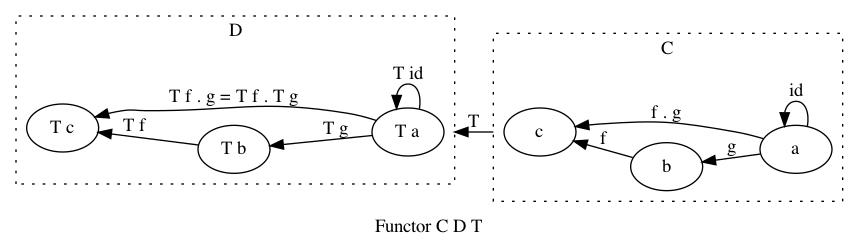
\includegraphics[width=.9\linewidth]{images/functor.png}
\end{center}

所以大部分把函子或者单子比喻成盒子其实在定义上是错的,虽然这样比喻比较容易理解,在使用上问题也不大。但是,函子只是从一个范畴到另一个范畴的箭头而已。

\begin{itemize}
\item 范畴间东西的函子标记为 \texttt{T(O)}
\item 范畴间箭头的函子标记为 \texttt{T(\textasciitilde{}>)}
\item 任何范畴 C 上存在一个 T 把所有的 O 和 \textasciitilde{}> 都映射到自己,标记为函子 1\textsubscript{C}
\begin{itemize}
\item 1\textsubscript{C}(O) = O
\item 1\textsubscript{C}(\textasciitilde{}>) = \textasciitilde{}>
\end{itemize}
\end{itemize}

\lstset{language=haskell,label= ,caption={函子的 Haskell 定义},captionpos=b,numbers=none}
\begin{lstlisting}
class (Category c, Category d) => Functor c d t where
  fmap :: c a b -> d (t a) (t b)
\end{lstlisting}

\lstset{language=scala,label= ,caption={函子的 Scala 定义},captionpos=b,numbers=none}
\begin{lstlisting}
trait Functor[C[_, _], D[_, _], T[_]]:
  def fmap[A, B](c: C[A, B]): D[T[A], T[B]]
\end{lstlisting}

\texttt{Functor c d t} 这表示从范畴 c 到范畴 d 的一个 Functor t

如果把范畴 c 和 d 都限制到 Hask 范畴:

\lstset{language=haskell,label= ,caption= ,captionpos=b,numbers=none}
\begin{lstlisting}
class Functor (->) (->) t where
  fmap :: (->) a b -> (->) (t a) (t b)
\end{lstlisting}

\lstset{language=scala,label= ,caption= ,captionpos=b,numbers=none}
\begin{lstlisting}
trait Functor[=>[_, _], =>[_, _], T[_]]:
 def fmap[A, B](c: =>[A, B]): =>[T[A], T[B]]
\end{lstlisting}

\texttt{->} 或者 \texttt{=>} 可以写在中间的:

这样就会变成我们熟悉的函子定义:\footnote{这里可以把 Functor 的第一第二个参数消掉, 因为已经知道是在 Hask 范畴了}

\lstset{language=haskell,label= ,caption= ,captionpos=b,numbers=none}
\begin{lstlisting}
class Functor t where
  fmap :: (a -> b) -> (t a -> t b)
\end{lstlisting}

\lstset{language=scala,label= ,caption= ,captionpos=b,numbers=none}
\begin{lstlisting}
trait Functor[T[_]]:
  def fmap[A, B](c: A => B): T[A] => T[B]
\end{lstlisting}

而 \emph{自函子/endofunctor} 就是这种连接相同范畴的 Functor,因为它从范畴 Hask 到达同样的范畴 Hask。
\index{endofunctor}
\index{自函子}

这回看代码就很容易对应上图和概念了, 这里的自函子只是映射范畴 \texttt{->} 到 \texttt{->}, 箭头函数那个箭头, 类型却变成了 \texttt{t a} 。

这里的 fmap 就是 T(\textasciitilde{}>),在 Hask 范畴上,所以是 T(->), 这个箭头是函数,所以也能表示成 T(f) 如果 \texttt{f:: a -> b}

\chapter{Cat/猫}
\label{sec:orgb23b488}

递归的, 当我们可以把一个范畴看成一个对象,函子看成箭头的话,那么我们又得到了一个新的范畴,这种对象是范畴箭头是函子的范畴我们叫它 -- \emph{Cat/猫} 。

已经没/meow的办法用语言描述这么高维度的事情了,请回忆\label{org0420545}并把 C 和 D 想象成点。

\chapter{自然变换 / Natural Transformations \label{org45b15a0}}
\label{sec:org7bc7d92}

函子是范畴间的映射,所以如果我们现在又把 Cat 范畴看成是对象, 那 Cat 范畴之间的箭头,其实就是函子的函子,
又升维度了,我们有个特殊的名字给它,叫 \sout{喵的变换} \emph{自然变换/Natural Transformations} 。
\index{Natural Transformations}
\index{自然变换}

\begin{figure}[htbp]
\centering
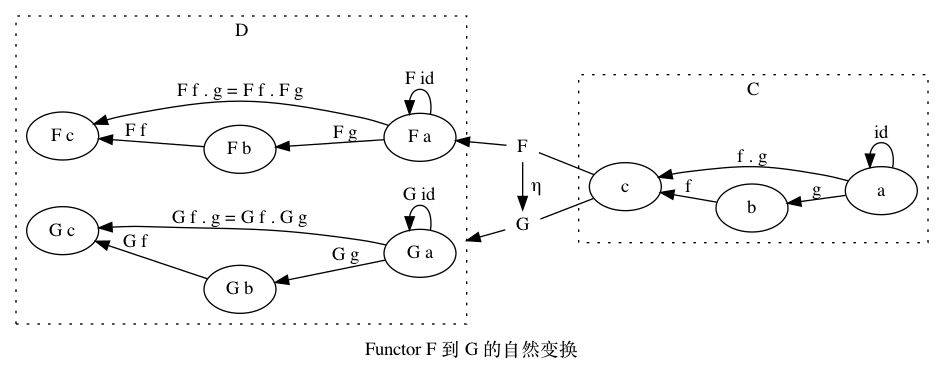
\includegraphics[width=.9\linewidth]{images/natrual-transformation.png}
\caption[Functor G \(\eta\)]{Functor F 和 G 以及 F 到 G 的自然变化}
\end{figure}


范畴 c 上的函子 f 到 g 的自然变化就可以表示成:
\lstset{language=haskell,label= ,caption= ,captionpos=b,numbers=none}
\begin{lstlisting}
type Nat c f g = c (f a) (g a)
\end{lstlisting}

Scala 3 的 rank n types\footnote{\url{https://blog.oyanglul.us/scala/dotty/en/rank-n-type} 别急, 后面马上讲到} 也很简洁:
\lstset{language=scala,label= ,caption= ,captionpos=b,numbers=none}
\begin{lstlisting}
type Nat[C[_,_],F[_],G[_]] = [A] => C[F[A], G[A]]
\end{lstlisting}

如果换到 Hask 范畴上的自然变化就变成了:

\lstset{language=haskell,label= ,caption= ,captionpos=b,numbers=none}
\begin{lstlisting}
type NatHask f g = f a -> g a
\end{lstlisting}

\lstset{language=scala,label= ,caption= ,captionpos=b,numbers=none}
\begin{lstlisting}
type Nat[F[_],G[_]] = [A] => F[A] => G[A]
\end{lstlisting}

这就是 Scala 中常见的 FunctionK\footnote{\url{https://blog.oyanglul.us/scala/dotty/en/functionk}}。

恭喜你到达 Functor 范畴.

当然, 要成为范畴,还有两个属性:
\begin{itemize}
\item id 为 f a 到 f a 的自然变换
\item 自然变换的组合
\end{itemize}

\begin{center}
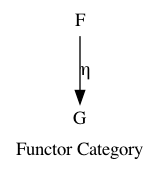
\includegraphics[width=.9\linewidth]{images/functor-category.png}
\end{center}

别着急, 我们来梳理一下,如果已经不知道升了几个维度了,我们假设类型所在范畴是第一维度
\begin{itemize}
\item 一维: Hask, 东西是类型,箭头是 ->
\item 二维: Cat, 东西是 Hask, 箭头是 Functor
\item 三维: Functor范畴, 东西是Functor, 箭头是自然变换
\end{itemize}

感觉到达三维已经是极限了,尼玛还有完没完了,每升一个维度还要起这么多装逼的名字,再升维度老子就画不出来了。

所以,是时候引入真正的技术了 -- String Diagram。

\chapter{String Diagram}
\label{sec:orga9ad355}

String Diagram\footnote{\url{https://www.youtube.com/watch?v=kiXjcqxVogE\&list=PL50ABC4792BD0A086\&index=5}} 的概念很简单,就是点变线线变点。

还记得当有了自然变换之后,三个维度已经没法表示了,那原来的点和线都升一维度,变成线和面,这样,就腾出一个点来表示自然变换了。

\begin{figure}[htbp]
\centering
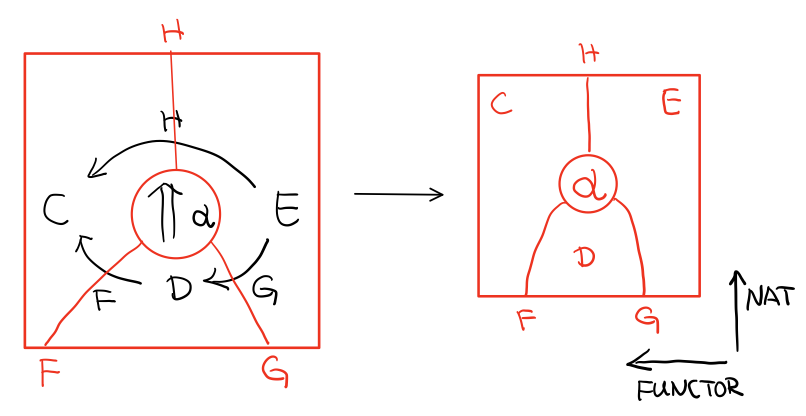
\includegraphics[width=.9\linewidth]{images/p1-string-diagram.png}
\caption{String Diagram:自然变换是点,函子是线,范畴是面,自然变换是点}
\end{figure}

组合(compose)的方向是从右往左,从下到上。

阅读起来,你会发现左右图给出的信息是完全等价的:
\begin{enumerate}
\item 范畴 E 通过 函子 D 到范畴 D,范畴 D 通过函子 F 到范畴 C
\item 范畴 E 通过 函子 E 到范畴 C
\item F . G 通过自然变换 \(\alpha\) 到 H
\end{enumerate}

\chapter{Adjunction Functor 伴随函子}
\label{sec:orgda3fd5f}
\index{Adjunction Functor}
伴随函子是范畴 C 和 D 之间有来有回的函子,为什么要介绍这个,因为它直接可以推出单子。

让我们来看看什么叫有来回。

\begin{center}
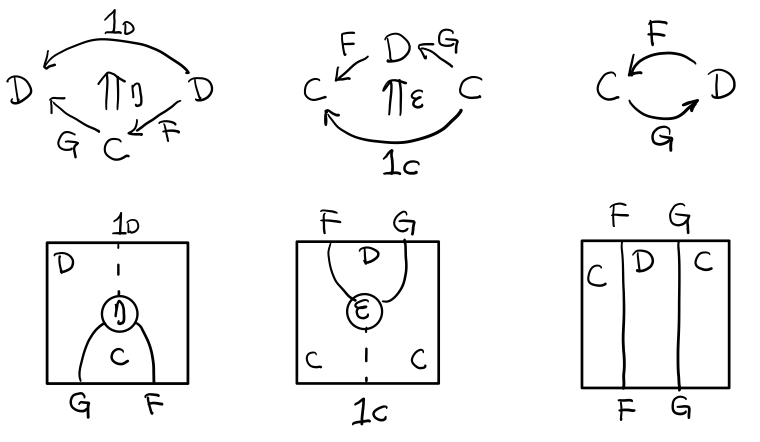
\includegraphics[width=.9\linewidth]{images/p1-adjunction-functor.png}
\end{center}

其中:

\begin{itemize}
\item 图右:一个范畴 C 可以通过函子 G 到范畴 D,再通过函子 F 回到 C,那么 F 和 G 就是伴随函子。
\item 图中:范畴 C 通过函子组合 F . G 回到范畴 C,函子 G . F 通过自然变换 \(\eta\) 到函子 1\textsubscript{D}
\item 图左:范畴 D 通过函子组合 G . F 回到范畴 D,函子 1\textsubscript{C} 通过自然变化 \(\epsilon\) 到函子 F . G
\end{itemize}

同时根据同构的定义,G 与 F 是 \emph{同构} 的。
\index{isomorphic}
\index{同构}

同构指的是若是有
\lstset{language=haskell,label= ,caption= ,captionpos=b,numbers=none}
\begin{lstlisting}
f :: a -> b
f':: b -> a
\end{lstlisting}

那么 f 与 f' 同构,因为 \texttt{f . f' = id = f' . f}

伴随函子的 F . G 组合是 C 范畴的 id 函子 \texttt{F . G = 1\_c}

\begin{figure}[htbp]
\centering
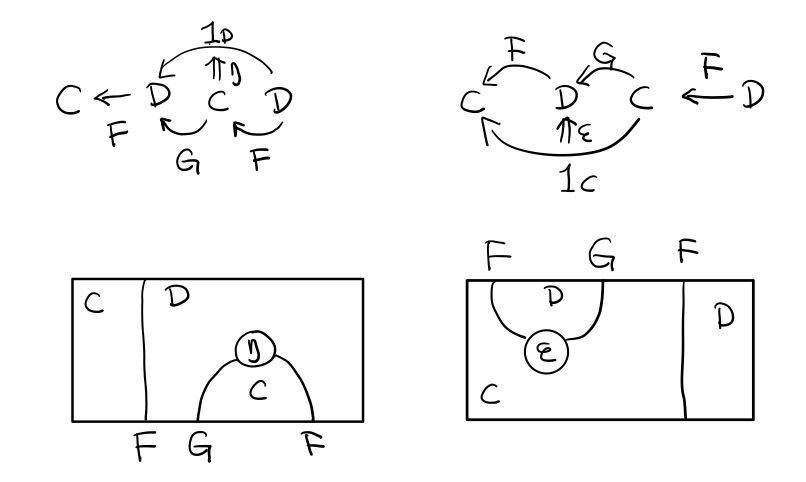
\includegraphics[width=.9\linewidth]{images/p1-ajunction-functor-compose.png}
\caption{伴随函子的两个Functor组合, 左侧记为 F eta, 右侧记为 epsilon F}
\end{figure}

注意看坐标,该图横着组合表示函子组合,竖着是自然变换维度,因此是自然变换的组合。

\begin{figure}[htbp]
\centering
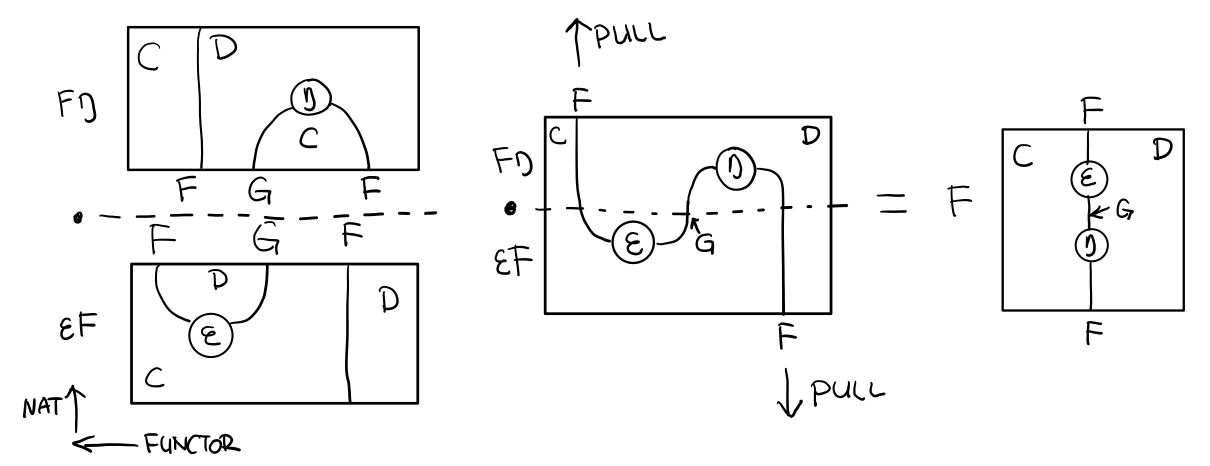
\includegraphics[width=.9\linewidth]{images/p1-ajunction-functor-compose-nat.png}
\caption{eta . epsilon = F -> F}
\end{figure}

当组合两个自然变换 \(\eta\) . \(\epsilon\) 得到一个弯弯曲曲的 F 到 F 的线时,我们可以拽着 F 的两端一拉,就得到了直的 F 线。

String Diagram 神奇的地方是所有线都可以拉上下两端,因为线不管是弯的还是直的,包含的信息并不会发生变化。
这个技巧非常有用,在之后的单子推导还需要用到。

\chapter{从伴随函子到 单子/Monad}
\label{sec:orga815b6c}
有了伴随函子,很容易推出单子,让我们先来看看什么是单子:

\begin{itemize}
\item 首先,它是一个自函子(endofunctor) T
\item 有一个从 i\textsubscript{c} 到 T 的自然变化 \(\eta\) (eta)
\item 有一个从 T\textsuperscript{2} 到 T 的自然变化 \(\mu\) (mu)
\end{itemize}

\begin{center}
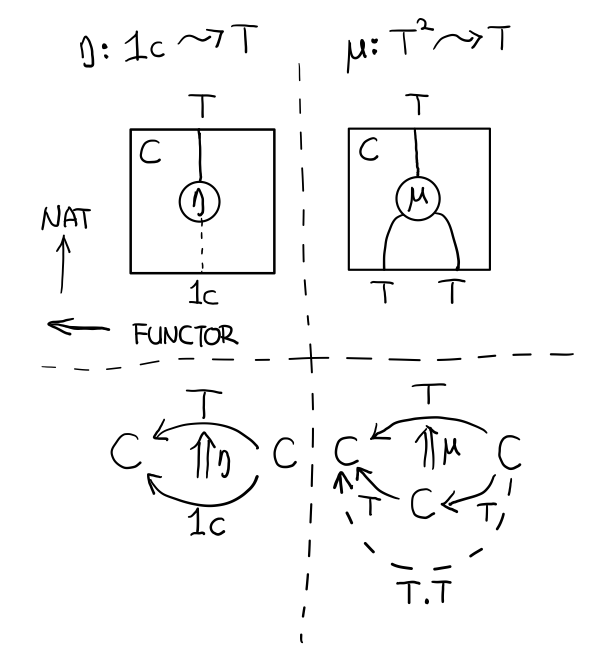
\includegraphics[width=.9\linewidth]{images/p1-monad-properties.png}
\end{center}

\lstset{language=haskell,label= ,caption= ,captionpos=b,numbers=none}
\begin{lstlisting}
class Endofunctor c t => Monad c t where
  eta :: c a (t a)
  mu  :: c (t (t a)) (t a)
\end{lstlisting}

\lstset{language=scala,label= ,caption= ,captionpos=b,numbers=none}
\begin{lstlisting}
trait Monad[C[_, _], T[_]]] extends Endofunctor[C, T]:
  def eta[A]: C[A, T[A]]
  def mu[A]: C[T[T[A]], T[A]]
\end{lstlisting}
同样,把 c = Hask 替换进去,就得到更类似我们 Haskell 中 Monad 的定义
\lstset{language=haskell,label= ,caption= ,captionpos=b,numbers=none}
\begin{lstlisting}
class Endofunctor m => Monad m where
  eta :: a -> (m a)
  mu :: m m a -> m a
\end{lstlisting}

\lstset{language=scala,label= ,caption= ,captionpos=b,numbers=none}
\begin{lstlisting}
trait Monad[M[_]] extends Endofunctor[M]:
  def eta[A]: A => M[A]
  def mu[A]: M[M[A]] => M[A]
\end{lstlisting}
要推出单子的 \(\eta\) 变换,只需要让 FG = T。可以脑补一下,因为是自函子,因此可以抹掉 D,
想象一下,当 D 这一块面被拿掉之后,线 F 和线 G 是不是就贴在一起了呢?两根贴着的线,不就是一根线吗?

\begin{figure}[htbp]
\centering
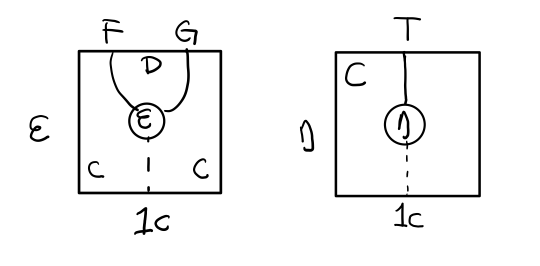
\includegraphics[width=.9\linewidth]{images/p1-ajunction-functor-to-monad-eta.png}
\caption{伴随函子的 epsilon 就是单子的 eta}
\end{figure}

同样的,当 FG = T, 也就是把 D 这陀给抹掉,F 和 G 就变成了 T。
\begin{figure}[htbp]
\centering
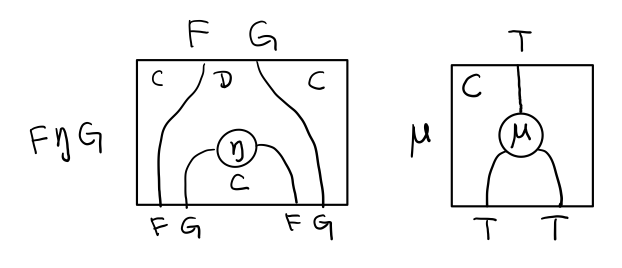
\includegraphics[width=.9\linewidth]{images/p1-ajunction-functor-to-monad-mu.png}
\caption{伴随函子的 F eta G 是函子的 mu}
\end{figure}

\section{三角等式}
\label{sec:org2d6499d}

三角等式是指 \(\mu\) . T \(\eta\) = T = \(\mu\) . \(\eta\) T

要推出三角等式只需要组合 F \(\eta\) G 和 \(\epsilon\) F G
\begin{figure}[htbp]
\centering
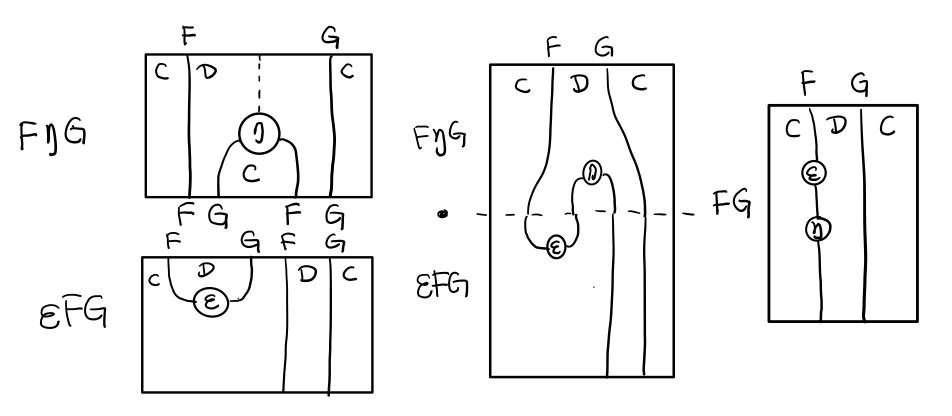
\includegraphics[width=.9\linewidth]{images/p1-adjunction-functor-triangle.png}
\caption{F eta G  . epsilon F G = F G}
\end{figure}
\begin{figure}[htbp]
\centering
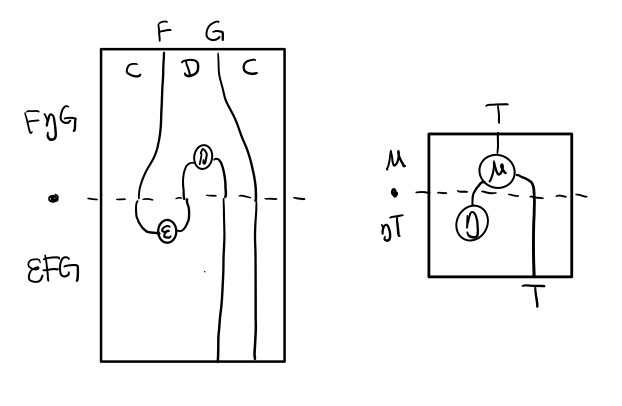
\includegraphics[width=.9\linewidth]{images/p1-monad-triangle.png}
\caption{F eta G  . epsilon F G= F G 对应到Monad就是 mu . eta T = T}
\end{figure}

换到代码上来说
\lstset{language=haskell,label= ,caption= ,captionpos=b,numbers=none}
\begin{lstlisting}
(mu . eta) m = m
\end{lstlisting}

同样的,左右翻转也成立

\begin{figure}[htbp]
\centering
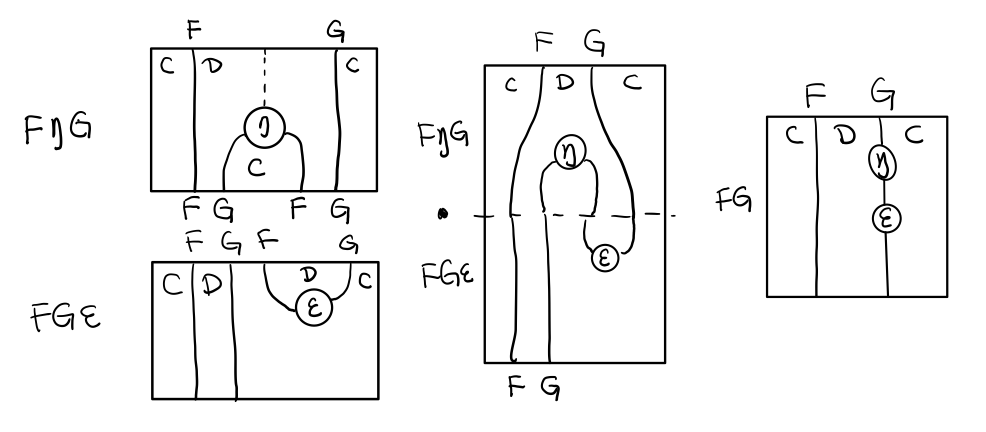
\includegraphics[width=.9\linewidth]{images/p1-adjunction-functor-triangle-reverse.png}
\caption{F eta G . F G epsilon = F G}
\end{figure}
\begin{figure}[htbp]
\centering
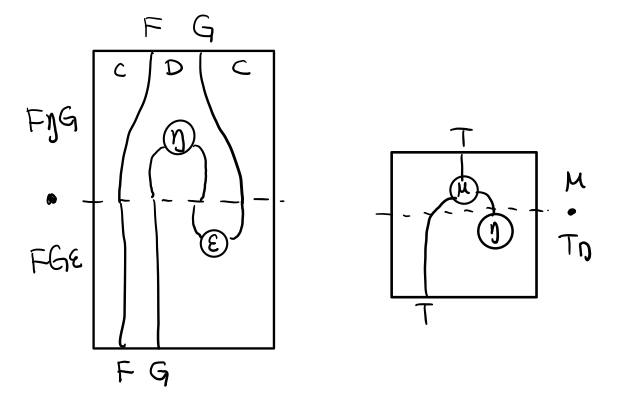
\includegraphics[width=.9\linewidth]{images/p1-monad-triangle-reverse.png}
\caption{F eta G . F G epsilon = F G 对应到 Monad是 mu . T eta = T}
\end{figure}
T \(\eta\) 就是 fmap eta
\lstset{language=haskell,label= ,caption= ,captionpos=b,numbers=none}
\begin{lstlisting}
(mu . fmap eta) m = m
\end{lstlisting}

如果把 \texttt{mu . fmap} 写成 \texttt{>>=} , 就有了

\lstset{language=haskell,label= ,caption= ,captionpos=b,numbers=none}
\begin{lstlisting}
m >>= eta = m
\end{lstlisting}

\section{结合律}
\label{sec:org3ad2f67}

单子另一大定律是结合律,让我们从伴随函子推起

假设我们现在有函子 F \(\eta\) G 和 函子 F \(\eta\) G F G, compose 起来会变成  F \(\eta\) G . F \(\eta\) G F G
\begin{center}
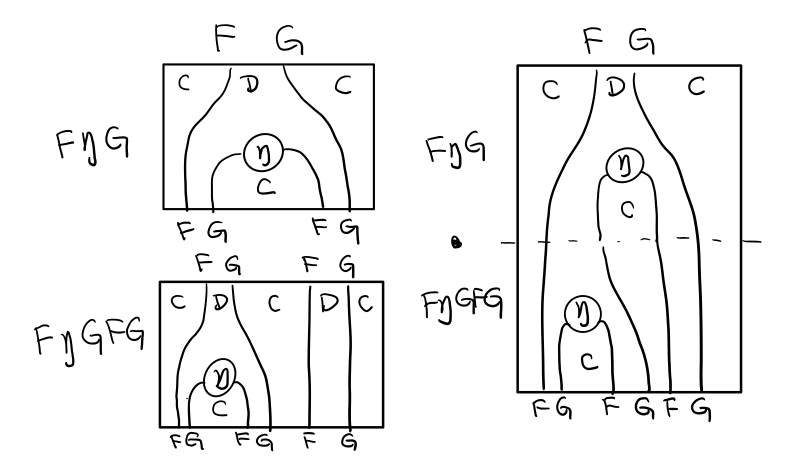
\includegraphics[width=.9\linewidth]{images/p1-ajunction-functor-monad-laws-1.png}
\end{center}

用 F G = T , F \(\eta\) G = \(\mu\) 代换那么就得到了单子的 \(\mu\) . \(\mu\) T
\begin{center}
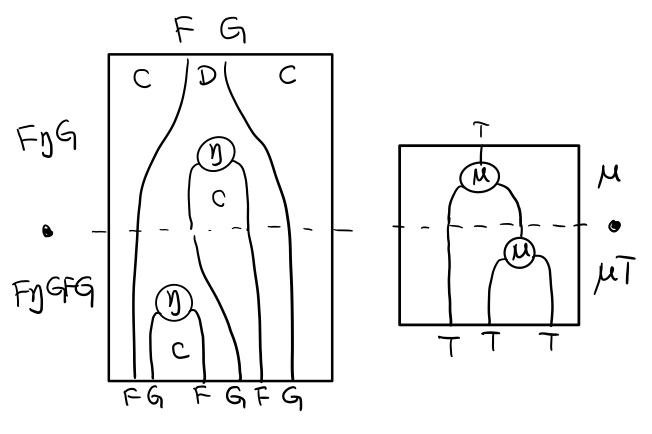
\includegraphics[width=.9\linewidth]{images/p1-ajunction-functor-monad-laws-2.png}
\end{center}

当组合 F \(\eta\) G 和 F G F \(\mu\) G 后,会得到一个镜像的图
\begin{center}
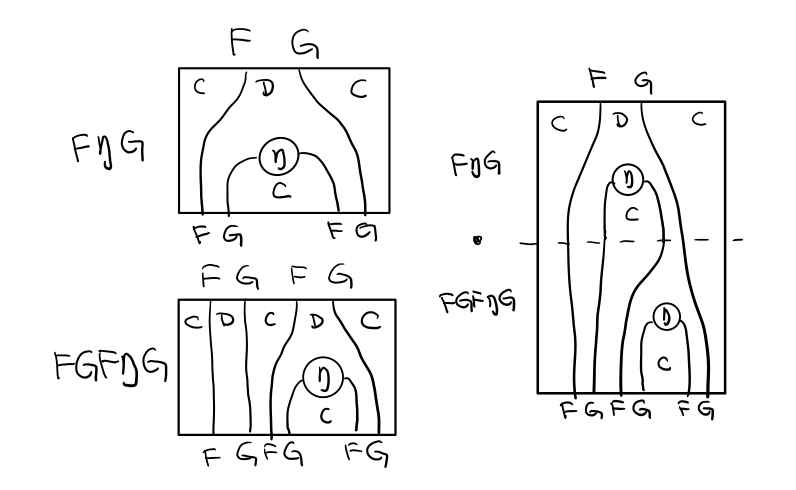
\includegraphics[width=.9\linewidth]{images/p1-ajunction-functor-monad-laws-3.png}
\end{center}

对应到单子的 \(\mu\) . T \(\mu\)

结合律是说 \(\mu\) . \(\mu\) T = \(\mu\) . T \(\mu\) , 即图左右翻转结果是相等的,为什么呢?看单子的String Diagram 不太好看出来,我们来看伴随函子

如果把左图的左边的 \(\mu\) 往上挪一点,右边的 \(\mu\) 往下挪一点,是不是跟右图就一样了
\begin{center}
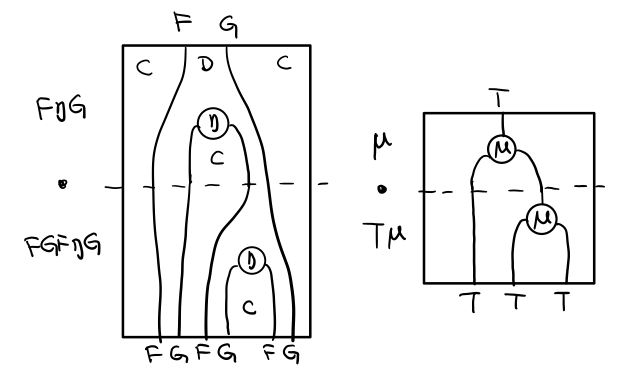
\includegraphics[width=.9\linewidth]{images/p1-ajunction-functor-monad-laws-4.png}
\end{center}

结合律反映到代码中就是
\lstset{language=haskell,label= ,caption= ,captionpos=b,numbers=none}
\begin{lstlisting}
mu . fmap mu = mu . mu
\end{lstlisting}

代码很难看出结合在哪里,因为正常的结合律应该是这样的 (1+2)+3 = 1+(2+3),但是不想加法的维度不一样,这里说的是自然变换维度的结合,可以通过String Diagram 很清楚的看见结合的过程,即 \(\mu\) 左边的两个T和先 \(\mu\) 右边两个 T 是相等的。

\chapter{Yoneda lemma / \sout{米田共} 米田引理}
\label{sec:orga68f251}
\index{米田引理}
\index{Yoneda Lemma}

米田引理是说所有的函子 \texttt{f a} 一定存在两个变换 \texttt{embed} 和 \texttt{unembed=,使得 =f a} 和 \texttt{(a -> b) -> F b} 同构。

要再 Haskell 中做到这一波操作需要先打开 \texttt{RankNTypes} 的编译器开关:

\lstset{language=haskell,label= ,caption= ,captionpos=b,numbers=none}
\begin{lstlisting}
{-# LANGUAGE RankNTypes #-}

embed :: Functor f => f a -> (forall b . (a -> b) -> f b)
embed x f = fmap f x

unembed :: Functor f => (forall b . (a -> b) -> f b) -> f a
unembed f = f id
\end{lstlisting}

Scala 3 不需要插件或者开关\footnote{\url{https://blog.oyanglul.us/scala/dotty/rank-n-type}},如果是 Scala 2 可以用 \texttt{apply} 来模拟. 比如 Cats 中 \href{https://typelevel.org/cats/datatypes/functionk.html}{FunctionK(\textasciitilde{}>)}。
\lstset{language=scala,label= ,caption= ,captionpos=b,numbers=none}
\begin{lstlisting}
type ~>[F[_],G[_]] = [A] => F[A] => G[A]
def embed[F[_], A](fa: F[A])(using F: Functor[F]) =
  [B] => (fn: A=>B) => f.fmap(fn)(fa)
def unembed[F[_]](fn: [B] => (A => B) => F[B]): F[A] =
  fn(identity)
\end{lstlisting}

\texttt{embed} 可以把 \texttt{f a} 变成 \texttt{(a -> b) -> f b}

\texttt{unembed} 是反过来, \texttt{(a -> b) -> f b} 变成 \texttt{f a}

上个图可能就明白了:
\begin{figure}[htbp]
\centering
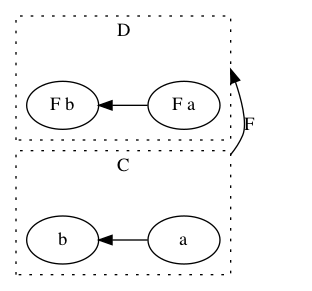
\includegraphics[width=.9\linewidth]{images/yoneda-lemma.png}
\caption{也就是说,图中无论知道a->b 再加上任意一个 F x,都能推出另外一个 F}
\end{figure}

这个引理看似很巧妙,特别是用 id 的这个部分,但是有什么用呢?

如果着急可以跳到 Free Monad/自由单子 部分,你会发现他是自由单子的基础。而且如果再往后会介绍的宇宙本原左看和右看,更会发现其中得精妙相似之处。

\section{Rank N Type}
\label{sec:orgbc21743}
\index{Arbitrary-rank polymorphism}
\index{Rank N Type}

前面说好的要解释 Rank N Type,这里赶快补充一下,不然等会我就忘了。

Haskell 中可以不用声明类型, 但是其实是省略掉 universally quantified \texttt{forall}, 如果把 forall 全部加回来,
就明了很多:

\begin{itemize}
\item Monomorphic Rank 0 / 0级单态\footnote{也就不是不变态}: t
\item Polymorphic Rank 1 / 1级 \sout{变态} 多态: forall a b. a -> b
\item Polymorphic Rank 2 / 2级多态: forall c. (forall a b. a -> b) -> c
\item Polymorphic Rank 3 / 3级多态: forall d . (forall c . (forall a b . a -> b) -> c) -> d
\end{itemize}

看 rank 几只要数左边 forall 的个数就好了.

一级多态只锁定一次类型 a 和 b

二级多态可以分两次确定类型, 第一次确定 c, 第二次确定 a b

三级多台分三次: 第一次 d, 第二次 c, 第三次 a b

比如:

\lstset{language=haskell,label= ,caption= ,captionpos=b,numbers=none}
\begin{lstlisting}
rank2 :: forall b c . b -> c -> (forall a. a -> a) -> (b, c)
rank2 b c f = (f b, f c)

rank2 True 'a' id
-- (True, 'a')
\end{lstlisting}

\begin{itemize}
\item \texttt{f} 在 \texttt{f True} 时类型 \texttt{Boolean -> Boolean} 是符合 \texttt{forall a. a->a} 的
\item 与此同时 \texttt{f 'a'} 时类型确实是 \texttt{Char -> Char} 但也符合 \texttt{forall a. a->a}
\end{itemize}

看 Scala 的更简单,因为 Scala 不能省去 universally quantified,只需要数方括号即可。
最左边 \texttt{[B, C]} 是 rank1, \texttt{fn} 的类型里的 \texttt{[A]} 是 rank2。

\lstset{language=scala,label= ,caption= ,captionpos=b,numbers=none}
\begin{lstlisting}
def rank2[B, C](b: B, c: C)(fn: [A] => A => A): (B, C) =
  (fn(b), fn(c))

rank2(true, 'a')([A] => (a: A) => A)
\end{lstlisting}

如果不用rank2 而是只有 rank1 类型系统就懵逼了:
\lstset{language=haskell,label= ,caption= ,captionpos=b,numbers=none}
\begin{lstlisting}
rank1 :: forall a b c . b -> c -> (a -> a) -> (b, c)
rank1 b c f = (f b, f c)
\end{lstlisting}

\lstset{language=scala,label= ,caption= ,captionpos=b,numbers=none}
\begin{lstlisting}
def rank1[A, B, C](b: B, c: C)(fn: A => A): (B, C) =
  (fn(b), fn(c))
\end{lstlisting}

f 在 \texttt{f True} 是确定 a 是 Boolean,在rank1多态是时就确定了 \texttt{a -> a} 的类型一定是 \texttt{Boolean -> Boolean} ,
然后当看到 \texttt{f 'a'} 时类型就挂了,因为 \texttt{'a'} 不是 \texttt{Boolean} 。

\chapter{\emph{Kleisli Catergory}}
\label{sec:org97818f4}
\index{Kleisi Catergory}

函子/Functor 的范畴叫做 函子范畴/Functor Catergory, 自然变换是其箭头。那单子/Monad也可以定义一个范畴吗?\footnote{当然, 单子是自函子,所以也可以是自函子范畴}

是的, 这个范畴名字叫做 \sout{单子范畴}\footnote{怎么说也是函数式编程的核心,怎么可以叫的这么low这么直接} 可莱斯利范畴/Kleisli Catergory\footnote{这个是我瞎翻译的, 但是读出来就是这么个意思, 真的, 不骗你, 照这么读绝对装的一手好逼, 不会被嘲笑的},那么 Kleisli 的箭头是什么?

\begin{figure}[htbp]
\centering
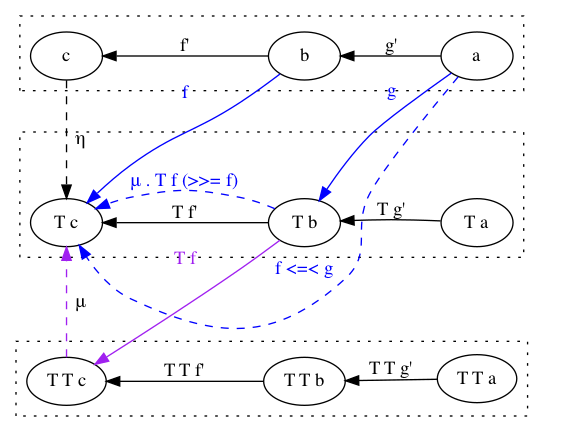
\includegraphics[width=.9\linewidth]{images/kleisli.png}
\caption[\sout{弯}]{注意观察大火箭 <=< 的轨迹, 不知道dot为什么会把这根线搞这么又弯又骚的, 和 >>= 。所以 Kleisli 其实就是斜着走的一个范畴,但是 >>= 把它硬生生掰 \sout{弯} 直了。}
\end{figure}

我们看定义,Kleisli Category:

\begin{enumerate}
\item 箭头是 Kleisli 箭头 \texttt{a -> T b}
\item 东西就是c范畴中的东西. 因为 a 和 b 都是 c 范畴上的, 由于T是自函子,所以 T b 也是 c 范畴的
\end{enumerate}

看到图上的 T f/ fmap f 和 \(\mu\) 了没?\footnote{(敲黑板) 就是紫色那根嘛!}

\lstset{language=haskell,label= ,caption= ,captionpos=b,numbers=none}
\begin{lstlisting}
f :: b -> T c
fmap f :: T b -> T T c
mu :: T T c -> T c
\end{lstlisting}

\lstset{language=scala,label= ,caption= ,captionpos=b,numbers=none}
\begin{lstlisting}
def f[T[_], B, C](b: B): T[C]
def fmap[T[_], B, C](f: B => C)(tb: T[B]): T[T[C]]
def mu[T[_], C](ttc: T[T[C]]): T[C]
\end{lstlisting}

紫色的箭头 \texttt{T f} \footnote{即 fmap f} 和紫色的虚线箭头 \(\mu\) 连起来就是 \texttt{T f'}, 那么最出名的 bind \texttt{>>=} 符号终于出来了:
\lstset{language=haskell,label= ,caption= ,captionpos=b,numbers=none}
\begin{lstlisting}
tb >>= f = (mu . fmap f) tb
\end{lstlisting}

Scala 中通常叫作 \texttt{flatMap} ,但如果你用 Cats 也是可以用 \texttt{>>=} 的。
\lstset{language=scala,label= ,caption= ,captionpos=b,numbers=none}
\begin{lstlisting}
def flatMap[T[_], B, C](f: B => T[C])(tb: T[B]): T[C] = (mu compose fmap(f))(tb)
\end{lstlisting}

下面这个大火箭 \texttt{<=<} 可以把蓝色箭头组合起来.
\lstset{language=haskell,label= ,caption= ,captionpos=b,numbers=none}
\begin{lstlisting}
(f <=< g) = mu . T f . g = mu . fmap f . g
\end{lstlisting}

\lstset{language=scala,label= ,caption= ,captionpos=b,numbers=none}
\begin{lstlisting}
def <=<[T[_], A, B, C](f: B => T[C])(g: A => T[B]): A => T[C] =
  mu compose fmap(f) compose g
\end{lstlisting}

因此大火箭就是 Kleisli 范畴的 \texttt{compose}

\lstset{language=haskell,label= ,caption= ,captionpos=b,numbers=none}
\begin{lstlisting}
(<=<) :: Monad T => (b -> T c) -> (a -> T b) -> (a -> T c)
\end{lstlisting}

\chapter{Summary}
\label{sec:orgd5dd7d5}
第一部分理论部分都讲完了, 如果你读到这里还没有被这些吊炸天/乱七八糟的概念劝退,
那么你这份如此强大得信念感,其实到后面两部分也不会有什么用。
因为,接下来的例子会很简单,我们要通过编程中常遇到的场景看看理论到底该如何得到实践?

\part{食用猫呢/Practical Monads}
\label{sec:orgee41947}

\begin{center}
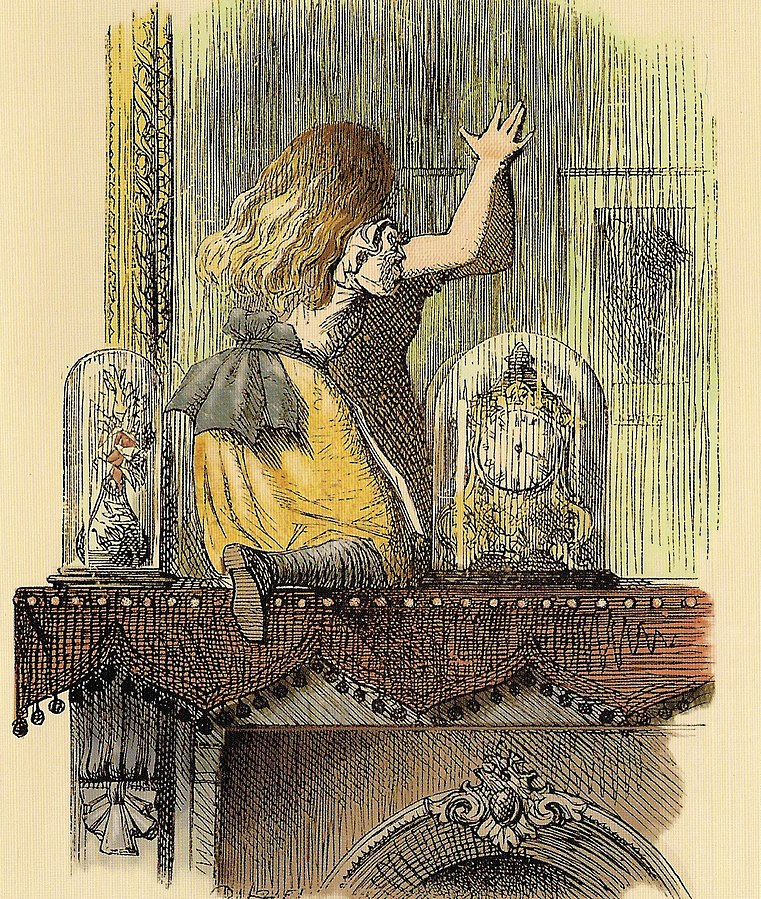
\includegraphics[width=.9\linewidth]{./images/Alice_through_the_looking_glass.jpg}
\end{center}

\chapter{Functor 食用函子定义}
\label{sec:org5fdf827}
\lstset{language=haskell,label= ,caption= ,captionpos=b,numbers=none}
\begin{lstlisting}
class Functor f where
  fmap :: (a -> b) -> (f a -> f b)
  (<$) :: a -> f b -> f a
  (<$) =  fmap . const
\end{lstlisting}

\lstset{language=scala,label= ,caption= ,captionpos=b,numbers=none}
\begin{lstlisting}
trait Functor[F[_]]:
  def fmap[A, B](fn: A => B): F[A] => F[B]
  extension [B](fb: F[B])
    def <$(a: A)(fb: F[B]): F[A] = fmap(const(a))
\end{lstlisting}

\chapter{Applicative}
\label{sec:orgd390c88}
\lstset{language=haskell,label= ,caption= ,captionpos=b,numbers=none}
\begin{lstlisting}
class Functor f => Applicative f where
  pure       :: a -> f a
  (<*>)      :: f (a -> b) -> f a -> f B
  liftA2     :: (a -> b -> c) -> f a -> f b -> f c
  liftA2 f x = (<*>) (fmap f x)
  (*>)       :: f a -> f b -> f b
  a1 *> a2   = (id <$ a1) <*> a2
  (<*)       :: f a -> f b -> f a
  (<*)       = liftA2 const
\end{lstlisting}

\lstset{language=scala,label= ,caption= ,captionpos=b,numbers=none}
\begin{lstlisting}
trait Applicative[F[_]] extends Functor[F]:
  def pure[A](a: A): F[A]
  def ap[A, B](fab: F[A=>B]): F[A] => F[B]
  def liftA2[A, B, C](f: A => B => C): F[A] => F[B] => F[C] = (x: F[A]) =>
    ap(fmap(f)(x))
  extension [A](fa: F[A])
    def *>(fb: F[B]) = (identity <$ fa) <*> fb
    def <*(fb: F[B]) = liftA2(const)
  extension [A, B](fab: F[A => B])
    def <*>(fa: F[B]) = ap(fab)(fa)
\end{lstlisting}

\chapter{Monad}
\label{sec:org3cf4122}
\lstset{language=haskell,label= ,caption= ,captionpos=b,numbers=none}
\begin{lstlisting}
class Applicative m => Monad m where
 (>>=)       :: forall a b. m a -> (a -> m b) -> m b
 (>>)        :: forall a b. m a -> m b -> m b
 m >> k      = m >>= \_ -> k
 return      :: a -> m a
 return      = pure
\end{lstlisting}

\lstset{language=scala,label= ,caption= ,captionpos=b,numbers=none}
\begin{lstlisting}
trait Monad[M[_]] extends Applicative[M] {
  def flatMap[A, B](ma: M[A])(f: A => M[B]): M[B]
  extension [A, B](ma: M[A])
    def >>(mb: M[B]): MB = flatMap(ma)((_: A) => mb)
}
\end{lstlisting}
\chapter{Identity 本身就有}
\label{sec:org4276978}

本身就有单子/ Identity Monad\footnote{从来没见过有人给这些数据类型按过中文名字, 不然我来, 这样也更好的体会这些数据类型的意图.} 可能是最简单的单子了。本身不包含任何计算, 且只有一个构造器:
\lstset{language=haskell,label= ,caption= ,captionpos=b,numbers=none}
\begin{lstlisting}
newtype Identity a = Identity { runIdentity :: a }
\end{lstlisting}

\lstset{language=scala,label= ,caption= ,captionpos=b,numbers=none}
\begin{lstlisting}
case class Identity[A](run: A)
\end{lstlisting}

\begin{itemize}
\item 这里取名 \texttt{Identity} 叫 \textbf{本身就有} ,所以 \texttt{Identity a} 就是 \textbf{本身就有 a}
\item 这里使用 \texttt{newtype} 而不是 \texttt{data} 是因为 \texttt{Identity} 与 \texttt{runIdentity} 是 \emph{同构} 的\footnote{见 \href{part1.org}{第一部分 伴随函子}}.
\end{itemize}

\lstset{language=haskell,label= ,caption= ,captionpos=b,numbers=none}
\begin{lstlisting}
Identity :: a -> Identity a
runIdentity :: Identity a -> a
\end{lstlisting}

你看 \texttt{runIdentity . Identity = id} ,所以他们是同构的。

左边的 \texttt{Identity} 是 \emph{类型构造器}\footnote{也就是 Kind * -> *, 因为它非常的 nice, 一定要等到 a 才出类型}, 接收类型 \texttt{a} 返回 \texttt{Identity a} 类型。

如果 \texttt{a} 是 \texttt{Int}, 那么就得到一个 \texttt{Identity Int} 类型。

右边的 \texttt{Identity} 是数据构造器,也就是构造值,比如 \texttt{Identity 1} 会构造出一个值,其类型为 \texttt{Identity Int} 。

大括号比较诡异,可以想象成给 \texttt{a} 自动生成了一个 \texttt{Identity a -> a} 的函数, 比如:

\lstset{language=haskell,label= ,caption= ,captionpos=b,numbers=none}
\begin{lstlisting}
runIdentity (Identity 1)
\end{lstlisting}

\lstset{language=scala,label= ,caption= ,captionpos=b,numbers=none}
\begin{lstlisting}
Identity(1).run
\end{lstlisting}

会返回 1

\textbf{本身就有} 可以实现 Functor 和 Monad,就得到 Identity 函子 和 Identity 单子。

\lstset{language=haskell,label= ,caption= ,captionpos=b,numbers=none}
\begin{lstlisting}
instance Functor Identity where
  fmap f (Identity a) = Identity (f a)

instance Monad Identity where
  return a = Identity a
  Identity a >>= f = f a
\end{lstlisting}

而 Scala 则用 \texttt{given} 来实现 typeclass:

\lstset{language=scala,label= ,caption= ,captionpos=b,numbers=none}
\begin{lstlisting}
given Functor[Identity]:
  def fmap[A, B](f: A => B): Identity[A] => Identity[B] =
    case Identity(a) => Identity(f(a))

given Monad[Identity]:
  def pure[A](a: A): Id[A] = Identity(a)
  def flatMap[A, B](f: A => Identity[B]): Identity[A] => Identity[B] =
    case Identity(a) => f(a)
\end{lstlisting}

可以看到 \texttt{Identity} 即是构造器/constructor,也是解构器/destructure,利用模式匹配是可以解构出值的。

上面函子实现中的 \texttt{fmap f (Identity a)}, 假如 \texttt{fmap} 的是 \texttt{Identity 1},
那么这个模式匹配到 \texttt{(Identity a)} 时会通过解构器把 \texttt{1} 放到 \texttt{a} 的位置。

\textbf{本来就有} 看起来什么也没有干,就跟 \texttt{identity} 函数一样,但是实际上, 它也跟 identity 相对于函数一样,在某些场景底下非常有用,比如后一部分搞基猫呢会
提的高达猫。

\chapter{Maybe 可能会有}
\label{sec:org038ba9f}
可能会有单子/Maybe Monad是一个超级简单的但比本身就有稍稍复杂的单子.

因为它拥有比本身就有多一个的类型构造器,类似这样的叫做 代数数据类型/ Algebra Data Type(ADT)

\lstset{language=haskell,label= ,caption= ,captionpos=b,numbers=none}
\begin{lstlisting}
data Maybe a = Just a | Nothing
\end{lstlisting}

其中 \texttt{a} \footnote{一定要记得小写哦}表示是任意类型.

你看, 不管是 \texttt{Just} 还是 \texttt{Nothing} 都可以构造出一个 \texttt{Maybe} 类型的数据来.

ADT 在 Scala 可以用 enum 表示, 而且, Scala 中的 \texttt{Maybe} 叫做 \texttt{Option}:

\lstset{language=scala,label= ,caption= ,captionpos=b,numbers=none}
\begin{lstlisting}
enum Option[+A]:
  case Some(a: A)
  case None
\end{lstlisting}


所以 \texttt{Just 1} 会得到一个 \texttt{Num a => Mabye a} 类型\footnote{意思就是 \texttt{Maybe a} 但是 \texttt{a} 的类型约束为 \texttt{Num}},
\texttt{Nothing} 也会得到一个 \texttt{Maybe a} 只不过 \texttt{a} 没有类型约束。

总之我们有了构造器可以构造出 \texttt{Maybe} 类型,而这个类型能做的事情,就要取决它实现了哪些 typeclass 的实例 了。比如它可以是一个函子.
\lstset{language=haskell,label= ,caption= ,captionpos=b,numbers=none}
\begin{lstlisting}
instance Functor Maybe where
  fmap f (Just a) = Just (f a)
  fmap f Nothing = Nothing
\end{lstlisting}

\lstset{language=scala,label= ,caption= ,captionpos=b,numbers=none}
\begin{lstlisting}
given Functor[Option]:
  def fmap[A, B](f: A => B): Option[A] => Option[B] =
    case Some(a) => Some(f(a))
    case None => None
\end{lstlisting}

\begin{figure}[htbp]
\centering
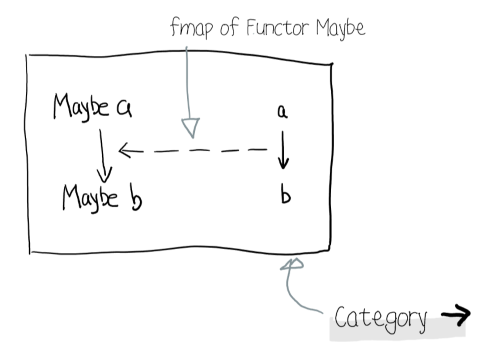
\includegraphics[width=.9\linewidth]{images/p2-maybe-functor.png}
\caption{fmap :: (a -> b) -> f a -> f b}
\end{figure}

看清楚了, 虚线箭头即 \texttt{fmap}, 图上表示的 \texttt{fmap} 是 \texttt{(a -> b) - - -> (Maybe a -> Maybe b)} 由于这里的箭头都是在 \texttt{->} 范畴, 所以 \texttt{- - ->} 就是 \texttt{->} 了.

即: \texttt{fmap :: (a -> b) -> f a -> f b}

不仅如此,还可以实现单子:
\lstset{language=haskell,label= ,caption= ,captionpos=b,numbers=none}
\begin{lstlisting}
instance Monad Maybe where
  return a = Just a
  (Just a) >>= f = f a
  Nothing >>= f = Nothing
\end{lstlisting}

\lstset{language=scala,label= ,caption= ,captionpos=b,numbers=none}
\begin{lstlisting}
given Monad[Option]:
  def pure[A](a: A): Option[A] = Some(a)
  def flatMap[A, B](f: A => Option[B]): Option[A] => Option[B] =
    case Some(a) => f(a)
    case None => None
  extension [A,B](fa: Option[A])
    def >>=(f: A => Option[B]): Option[B] = flatMap(f)(fa)
\end{lstlisting}

\begin{figure}[htbp]
\centering
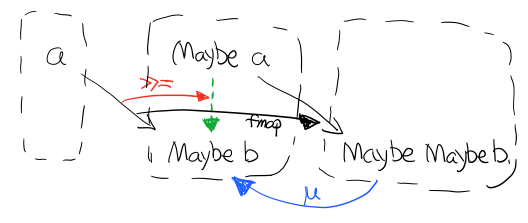
\includegraphics[width=.9\linewidth]{images/p2-maybe-kleisli.png}
\caption{还记得第一部分提到的 Kleisli 范畴吗?}
\end{figure}

Maybe 有用在于能合适的处理 \emph{偏函数} Partial Function/ 的返回值。
偏函数相对于 \emph{全函数} Total Function/ 是指只能对部分输入返回输出的函数。

比如一个取数组某一位上的值的函数,就是偏函数,因为假设你想取第4位的值,但不是所有数组长度都大于4,就会有获取不了的尴尬情况。
\lstset{language=haskell,label= ,caption= ,captionpos=b,numbers=none}
\begin{lstlisting}
[1,2,3] !! 4
\end{lstlisting}

\lstset{language=scala,label= ,caption= ,captionpos=b,numbers=none}
\begin{lstlisting}
List(1,2,3).get(4)
\end{lstlisting}

如果使用 Maybe 把偏函数处理不了的输入都返回成 Nothing,这样结果依然保持 Maybe 类型,不影响后面的计算。

\lstset{language=haskell,label= ,caption= ,captionpos=b,numbers=none}
\begin{lstlisting}
([[1,2,3], [4,5,6]] !! 1) >>= \x -> x !! 2
\end{lstlisting}

\lstset{language=scala,label= ,caption= ,captionpos=b,numbers=none}
\begin{lstlisting}
List(List(1,2,3), List(4,5,6)).get(1) >>= { _.get(2) }
\end{lstlisting}

\chapter{Either 要么有要么有}
\label{sec:org542b817}

Either 的定义也很简单
\lstset{language=haskell,label= ,caption= ,captionpos=b,numbers=none}
\begin{lstlisting}
data Either a b = Left a | Right b
\end{lstlisting}

\lstset{language=scala,label= ,caption= ,captionpos=b,numbers=none}
\begin{lstlisting}
enum Either[+A, +B]:
  case Left(a: A)
  case Right(b: B)
\end{lstlisting}


\section{Product \& Coproduct}
\label{sec:orgb971bb5}
看过第一部分应该还能记得有一个东西叫 Duel,所以见到如果范畴上有 Coproduct 那么肯定在duel范畴上会有同样的东西叫 Product。

那么我们先来看看什么是 Coproduct

\begin{figure}[htbp]
\centering
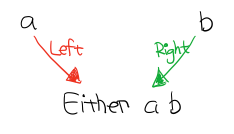
\includegraphics[width=.9\linewidth]{images/p2-coproduct.png}
\caption{Coproduct}
\end{figure}

像这样,能通过两个箭头到达同一个东西,就是 Coproduct。这里箭头 \texttt{Left} 能让 \texttt{a} 到 \texttt{Either a b} , 箭头 \texttt{Right} 也能让 \texttt{b} 到达 \texttt{Either a b}

有意思的是还肯定存在一个 Coproduct 和 箭头,使得下图成立
\begin{center}
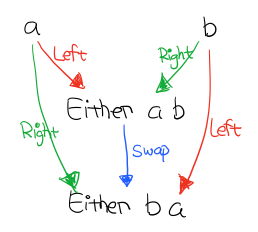
\includegraphics[width=.9\linewidth]{images/p2-coproduct-law.png}
\end{center}

箭头反过来,就是 Product, 比如 Tuple

\begin{figure}[htbp]
\centering
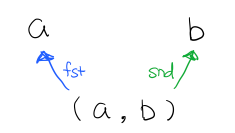
\includegraphics[width=.9\linewidth]{images/p2-product.png}
\caption{Product}
\end{figure}

Tuple 的 \texttt{fst} 箭头能让 \texttt{(a, b)} 到达 \texttt{a} 对象,而箭头 \texttt{snd} 能让其到达 \texttt{b} 对象。

\section{Either Monad}
\label{sec:org6b6ad30}
确切的说,Either 不是 monad, \texttt{Either a} 才是。还记得 monad 的 class 定义吗?
\lstset{language=haskell,label= ,caption= ,captionpos=b,numbers=none}
\begin{lstlisting}
class Endofunctor m => Monad m where
  eta :: a -> (m a)
  mu :: m m a -> m a
\end{lstlisting}
所以 m 必须是个 Endofunctor,也就是要满足 Functor
\lstset{language=haskell,label= ,caption= ,captionpos=b,numbers=none}
\begin{lstlisting}
class Functor t where
  fmap :: (a -> b) -> (t a -> t b)
\end{lstlisting}
t a 的 kind 是 *,所以 t 必须是 kind * -> *
也就是说,m 必须是接收一个类型参数的类型构造器

而 Either 的 kind 是 * -> * -> *, Either a 才是 * -> *

所以只能定义 Either a 的 Monad
\lstset{language=haskell,label= ,caption= ,captionpos=b,numbers=none}
\begin{lstlisting}
instance Monad (Either a) where
  Left  l >>= _ = Left l
  Right r >>= k = k r
\end{lstlisting}

\lstset{language=scala,label= ,caption= ,captionpos=b,numbers=none}
\begin{lstlisting}
given [A]: Monad[Either[A, ?]] with
  def flatMap[B, C](f: B => Either[A, C]): Either[A, B] => Either[A, C] = (fa: Either[A, B]) =>
    fa match
      case Left(l) => Left(l)
      case Right(r) => f(r)
\end{lstlisting}

很明显的,>>= 任何函数到左边/ Left 都不会改变,只有 >>= 右边才能产生新的计算。

\chapter{Reader 差一点就有}
\label{sec:orge52651d}

\emph{差一点就有} 的作用是描述一个需要喂数据的计算。

在描述计算的时候,并不需要关心具体输入的值是什么,更需要关注的是输入的类型。
当计算需要以来该值时,只需要 asks 就可以假装拿到输入值,继续描述接下来的计算。

而真正的输入,会在最终运行计算时给予。

跟 \emph{本身就有} 一样,我们用 newtype 来定义一个同构的 \emph{差一点就有} 类型:

\lstset{language=haskell,label= ,caption= ,captionpos=b,numbers=none}
\begin{lstlisting}
newtype Reader e a = Reader { runReader :: (e -> a) }
\end{lstlisting}

\lstset{language=scala,label= ,caption= ,captionpos=b,numbers=none}
\begin{lstlisting}
case class Reader[E, A](run: E => A)
\end{lstlisting}

其中:
\begin{itemize}
\item e 是输入
\item a 是结果
\item 构造 Reader 类型需要确定输入的类型 e 与输出的类型 a
\item \texttt{runReader} 的类型是 \texttt{runReader:: (Reader e a) -> (e -> a)}
\end{itemize}

也就是说在描述完一个 Reader 的计算后,使用 runReader 可以得到一个 e -> a 的函数,使用这个函数,就可以接收输入,通过构造好的计算,算出结果 a 返回。

那么,让我们来实现 Reader 的单子实力,就可以描述一个可以 ask 的计算了。

\lstset{language=haskell,label= ,caption= ,captionpos=b,numbers=none}
\begin{lstlisting}
instance Monad (Reader e) where
    return a         = Reader $ \_ -> a
    (Reader g) >>= f = Reader $ \e -> runReader (f (g e)) e
\end{lstlisting}

\begin{verbatim}
given [E]: Monad[Reader[E, ?]] with
  def pure[A](a: A): Reader[E, A] = Reader((e: E) => a)
  def flatMap[A, B](f: A => Reader[E, B]): Reader[E, A] => Reader[E, B] = (fa: Reader[E, A]) =>
    Reader((e: E) => f(fa.run(e)).run(e)

\end{verbatim}

跟Either一样,我们只能定义 Reader e 的 monad instance。

注意这里的
\begin{itemize}
\item f 类型是 \texttt{(a -> Reader e a)}
\item g 其实就是是 destructure 出来的 runReader,也就是 e -> a
\item 所以 (g e) 返回 a
\item f (g e) 就是 \texttt{Reader e a}
\item 再 run 一把最后得到 a
\end{itemize}

\begin{figure}[htbp]
\centering
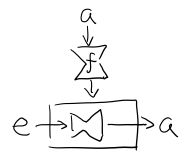
\includegraphics[width=.9\linewidth]{images/p2-reader-monad.png}
\caption{f 函数,接收 a 返回一个 从 e 到 a 的 Reader}
\end{figure}

让我们来看看如何使用 Reader
\lstset{language=haskell,label= ,caption= ,captionpos=b,numbers=none}
\begin{lstlisting}
import Control.Monad.Reader

data Environment = Env
  { fistName :: String
  , lastName :: String
  } deriving (Show)

helloworld :: Reader Environment String
helloworld = do
  f <- asks firstName
  l <- asks lastName
  return "Hello " ++ f ++ l

runHelloworld :: String
runHelloworld = runReader helloworld $ Env "Jichao" "Ouyang"
\end{lstlisting}

这段代码很简单,helloworld 负责打招呼,也就是在名字前面加个 "Hello",而跟谁打招呼,这个函数并不关心,而单纯的是向 Environment 问/asks 就好。

\begin{figure}[htbp]
\centering
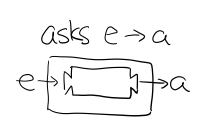
\includegraphics[width=.9\linewidth]{images/p2-reader-monad-ask.png}
\caption{asks 可以将 e -> a 的函数变换成 Reader e a}
\end{figure}

在运行时,可以提供给 Reader 的输入 Env fistname lastname。
\begin{center}
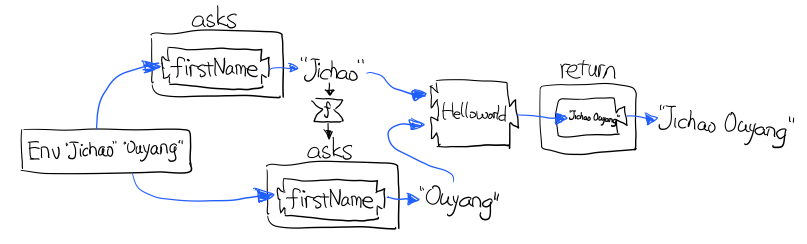
\includegraphics[width=.9\linewidth]{images/p2-reader-monad-run.png}
\end{center}

\section{do notation}
\label{sec:orgcd119be}
这可能是你第一次见到 \texttt{do} 和 \texttt{<-}. 如果不是,随意跳过这节。

\begin{itemize}
\item do 中所有 <- 的右边都是 \texttt{Reader Environment String} 类型
\item do 中的 return 返回类型也必须为  \texttt{Reader Environment String}
\item \texttt{asks firstName} 返回的是 \texttt{Reader Environment String} 类型, \texttt{<-} 可以理解成吧 monad \texttt{Reader Environment} 的内容放到左边的 f, 所以 f 的类型是 String。
\end{itemize}

看起来像命令式的语句,其实只是 \texttt{>>=} 的语法糖,但是明显用do可读性要高很多。
\lstset{language=haskell,label= ,caption= ,captionpos=b,numbers=none}
\begin{lstlisting}
helloworld = (asks firstName) >>=
  \f -> (asks lastName) >>=
       \l -> return "Hello " ++ f ++ l
\end{lstlisting}


\chapter{Writer 光出进没有}
\label{sec:org97934f2}

除了返回值,计算会需要产生一些额外的数据,比如 log

此时就需要一个 Writter,其返回值会是一个这样 \texttt{(result, log)} 的 tuple

限制是 log 的类型必须是个 含幺半群/monoid

\lstset{language=haskell,label= ,caption= ,captionpos=b,numbers=none}
\begin{lstlisting}
example :: Writer String String
example  = do
  tell "How are you?"
  tell "I'm fine thank you, and you?"
  return "Hehe Da~"

output :: (String, String)
output = runWriter example
-- ("Hehe Da~", "How are you?I'm fine thank you, and you?")
\end{lstlisting}

Writer 的定义更简单
\lstset{language=haskell,label= ,caption= ,captionpos=b,numbers=none}
\begin{lstlisting}
newtype Writer l a = Writer { runWriter :: (a,l) }
\end{lstlisting}
里面只是一个 tuple 而已
\begin{itemize}
\item w 是 log
\item a 是 返回值
\end{itemize}

看看如何实现 Writer monad
\lstset{language=haskell,label= ,caption= ,captionpos=b,numbers=none}
\begin{lstlisting}
instance (Monoid w) => Monad (Writer w) where
    return a             = Writer (a,mempty)
    (Writer (a,l)) >>= f = let (a',l') = runWriter $ f a in
                           Writer (a',l `mappend` l')
\end{lstlisting}

\begin{itemize}
\item return 不会有任何 log,l 是 monoid 的 mempty
\item f 的类型为 \texttt{a -> Writer l a}
\item \texttt{runWriter \$ f a} 返回 \texttt{(a, l)}
\end{itemize}

\begin{center}
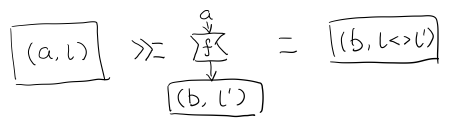
\includegraphics[width=.9\linewidth]{images/p2-writer-monad.png}
\end{center}

所以在 >>= 时,我们先把 f a 返回的 Writer run了,然后把两次 log \texttt{mappend} 起来。
\begin{center}
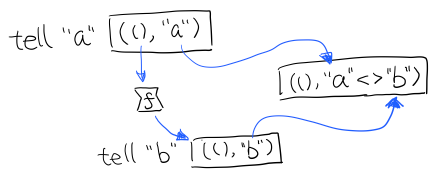
\includegraphics[width=.9\linewidth]{images/p2-writer-monad-bind.png}
\end{center}

\chapter{State 变化会有}
\label{sec:org4cf833a}
跟名字就看得出来 State monad 是为了处理状态。虽然函数式编程不应该有状态,不然会引用透明性。但是,state monad并不是在计算过程中修改状态,而是通过描述这种变化,然后需要时在运行返回最终结果。这一点跟 Reader 和 Writer 这两个看起来是副作用的 IO 是一样的。

先看下 State 类型的定义
\lstset{language=haskell,label= ,caption= ,captionpos=b,numbers=none}
\begin{lstlisting}
newtype State s a = State { runState :: s -> (a, s) }
\end{lstlisting}

可以看到 State 只包含一个 从旧状态 s 到新状态 s 和返回值 a 的 Tuple 的函数。

通过实现 Monad,State 就可以实现命令式编程中的变量的功能。
\lstset{language=haskell,label= ,caption= ,captionpos=b,numbers=none}
\begin{lstlisting}
instance Monad (State s) where
  return a        = State $ \s -> (a,s)
  (State x) >>= f = State $ \s -> let (v,s') = x s in
                                 runState (f v) s'
\end{lstlisting}
return 很简单,就不用解释了。

\begin{center}
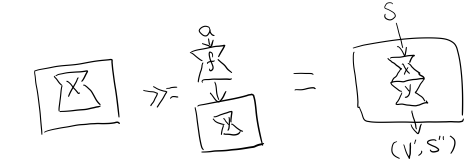
\includegraphics[width=.9\linewidth]{images/p2-state-monad.png}
\end{center}

x 类型是 \texttt{s -> (a, s)} ,所以 x s 之后会返回 结果和状态。也就是运行当前 State,把结果 v 传给函数 f,返回的 State 再接着上次状态运行。

\begin{figure}[htbp]
\centering
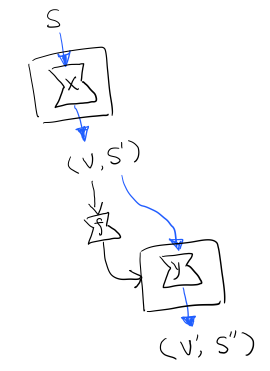
\includegraphics[width=.9\linewidth]{images/p2-state-monad-bind.png}
\caption{State x >>= f 后runState的数据流(啊啊啊,画歪了,感觉需要脉动一下)}
\end{figure}

使用起来也很方便,State 提供 \texttt{get} \texttt{put} \texttt{moidfy} 三个方便的函数可以生成修改状态的State monad

\lstset{language=haskell,label= ,caption= ,captionpos=b,numbers=none}
\begin{lstlisting}
import Control.Monad.Trans.State.Strict
test :: State Int Int
test = do
  a <- get
  modify (+1)
  b <- get
  return (a + b)

main = print $ show $ runState test 3
-- (7, 4)
\end{lstlisting}


\chapter{Validation 检查检查}
\label{sec:org811d64e}
如果你有注意到,前面的 Either 可以用在处理错误和正确的路径分支,但是问题是错误只发生一次。

\begin{quote}
Validation 没有在标准库中,但是我觉得好有用啊,你可以在 ekmett 的 \href{https://github.com/ekmett/either}{github} 中找到源码
\end{quote}

想象一下这种场景,用户提交一个表单,我们需要对每一个field进行验证,如果有错误,需要把错误的哪几个field的错误消息返回。显然如果使用 Either 来做,只能返回第一个field的错误信息,后面的计算都会被跳过。

针对这种情况, Validation 更适合
\lstset{language=haskell,label= ,caption= ,captionpos=b,numbers=none}
\begin{lstlisting}
data Validation e a = Failure e | Success a
\end{lstlisting}

ADT定义看起来跟 Either 是一样的,不同的是 左边/Left Failure 是 含幺半群/Monoid

\section{含幺半群/Monoid}
\label{sec:orgc6d7ebb}
monoid 首先得是 半群/Semigroup ,然后再 含幺。
\lstset{language=haskell,label= ,caption= ,captionpos=b,numbers=none}
\begin{lstlisting}
class Semigroup a where
  (<>) :: a -> a -> a
  (<>) = mappend
\end{lstlisting}

半群非常简单,只要是可以 \texttt{<>} (mappend) 的类型就是了。

含幺只需要有一个 \texttt{mempty} 的 幺元就行
\lstset{language=haskell,label= ,caption= ,captionpos=b,numbers=none}
\begin{lstlisting}
class Monoid a where
  mempty  :: a
  mappend :: a -> a -> a
\end{lstlisting}

比如 List 就是 Semigroup
\lstset{language=haskell,label= ,caption= ,captionpos=b,numbers=none}
\begin{lstlisting}
instance Semigroup [a] where
  (<>) = (++)
\end{lstlisting}
也是 Monoid
\lstset{language=haskell,label= ,caption= ,captionpos=b,numbers=none}
\begin{lstlisting}
instance Monoid [a] where
  mempty  = []
  mappend = (++)
\end{lstlisting}

Monoid 的 \texttt{<>} 满足:
\begin{itemize}
\item mempty <> a = a
\item a <> b <> c = a <> (b <> c)
\end{itemize}
\section{回到 Validation}
\label{sec:orgf1319d4}
现在让 Failure e 满足 Monoid,就可以 \texttt{mappend} 错误信息了。
\lstset{language=haskell,label= ,caption= ,captionpos=b,numbers=none}
\begin{lstlisting}
instance Semigroup e => Semigroup (Validation e a) where
  Failure e1 <> Failure e2 = Failure (e1 <> e2)
  Failure _  <> Success a2 = Success a2
  Success a1 <> Failure _  = Success a1
  Success a1 <> Success _  = Success a1
\end{lstlisting}

下来,我们用一个简单的例子来看看 Validation 与 Either 有什么区别。

假设我们有一个form,需要输入姓名与电话,验证需要姓名是非空而电话是11位数字。

首先,我们需要有一个函数去创建包含姓名和电话的model
\lstset{language=haskell,label= ,caption= ,captionpos=b,numbers=none}
\begin{lstlisting}
data Info = Info {name: String, phone: String} deriving Show
\end{lstlisting}

然后我们需要验证函数
\lstset{language=haskell,label= ,caption= ,captionpos=b,numbers=none}
\begin{lstlisting}
notEmpty :: String -> String -> Validation [String] String
notEmpty desc "" = Failure [desc <> " cannot be empty!"]
notEmpty _ field = Success field
\end{lstlisting}
notEmpty 检查字符是否为空,如果是空返回 Failure 包含错误信息,若是非空则返回 Success 包含 field

同样的可以创建 11位数字的验证函数
\lstset{language=haskell,label= ,caption= ,captionpos=b,numbers=none}
\begin{lstlisting}
phoneNumberLength :: String -> String -> Validation [String] String
phoneNumberLength desc field | (length field) == 11 = Success field
                             | otherwise = Failure [desc <> "'s length is not 11"]
\end{lstlisting}
实现 Validation 的 Applicative instance,这样就可以把函数调用lift成带有验证的 Applicative
\lstset{language=haskell,label= ,caption= ,captionpos=b,numbers=none}
\begin{lstlisting}
instance Semigroup e => Applicative (Validation e) where
  pure = Success
  Failure e1 <*> Failure e2 = Failure e1 <> Failure e2
  Failure e1 <*> Success _  = Failure e1
  Success _  <*> Failure e2 = Failure e2
  Success f <*> Success a = Success (f a)
\end{lstlisting}
\begin{itemize}
\item 失败应用到失败会 concat 起来
\item 失败跟应用或被成功应用还是失败
\item 只有成功应用到成功才能成功,这很符合验证的逻辑,一旦验证中发生任何错误,都应该返回失败。
\end{itemize}

\lstset{language=haskell,label= ,caption= ,captionpos=b,numbers=none}
\begin{lstlisting}
createInfo :: String -> String -> Validation [String] Info
createInfo name phone = Info <$> notEmpty "name" name <*> phoneNumberLength "phone" phone
\end{lstlisting}

现在我们就可以使用带validation的 createInfo 来安全的创建 Info 了

\lstset{language=haskell,label= ,caption= ,captionpos=b,numbers=none}
\begin{lstlisting}
createInfo "jichao" "12345678910" -- Success Info "jichao" "12345678910"
createInfo "" "123" -- Failure ["name cannot be empty!", "phone's length is not 11"]
\end{lstlisting}

\chapter{Cont 接下来有}
\label{sec:orgba04a00}
Cont 是 Continuation Passing Style/CPS 的 monad,也就是说,它是包含 cps 计算 monad。

先看一下什么是 CPS,比如有一个加法
\lstset{language=haskell,label= ,caption= ,captionpos=b,numbers=none}
\begin{lstlisting}
add :: Int -> Int -> Int
add = (+)
\end{lstlisting}

但是如果你想在算法加法后,能够继续进行一个其他的计算,那么就可以写一个 cps版本的加法
\lstset{language=haskell,label= ,caption= ,captionpos=b,numbers=none}
\begin{lstlisting}
addCPS :: Int -> Int -> (Int -> r) -> r
addCPS a b k = k (a + b)
\end{lstlisting}

非常简单,现在我们可以看看为什么需要一个 Cont monad 来包住 CPS 计算,首先,来看 ADT 定义
\lstset{language=haskell,label= ,caption= ,captionpos=b,numbers=none}
\begin{lstlisting}
newtype Cont r a = Cont { runCont :: ((a -> r) -> r) }
\end{lstlisting}

又是一个同构的类型,Cont 构造器只需要一个 runCount,也就是让他能继续计算的一个函数。

完了之后来把之前的 addCPS 改成 Cont
\lstset{language=haskell,label= ,caption= ,captionpos=b,numbers=none}
\begin{lstlisting}
add :: Int -> Int -> Cont k Int
add a b = return (a + b)
\end{lstlisting}

注意到 addCPS 接收到 a 和 b 之后返回的类型是 \texttt{(Int -> r) -> r} ,而 Cont 版本的 \texttt{add} 返回 \texttt{Cont k Int}

明显构造 \texttt{Cont k Int} 也正是需要 \texttt{(Int -> r) -> r} ,所以 Cont 就是算了 k 的抽象了。

\lstset{language=haskell,label= ,caption= ,captionpos=b,numbers=none}
\begin{lstlisting}
instance Monad (Cont r) where
    return a = Cont ($ a)
    m >>= k  = Cont $ \c -> runCont m $ \a -> runCont (k a) c
\end{lstlisting}

\texttt{(\$ a)} 比较有意思, 我们都知道 \texttt{f \$ g a} 其实就是 \texttt{f(g a)}, 所以 \texttt{\$} 其实就是一个 apply 左边的函数到右边表达式的中缀函数, 如果写成前缀则是
\texttt{(\$ (g a) f)}. 是反的是因为 \texttt{\$} 是有结合, 需要右边表达式先求值, 所以只给一个 a 就相当于 \texttt{(\$ a) = \textbackslash{}f -> f a}

回到 Monad Cont\ldots{}

\chapter{Summary}
\label{sec:org539d46d}
第二部分食用部分也讲完了, 不知是否以及大致了解了monad的尿性各种基本玩法呢?通过这些常用的基本的 monad instance,解决命令式编程中的一些简单问题应该是够了。

不过,接下来还有更变态的猫,就先叫她 \sout{搞基} 猫呢好了。

\begin{itemize}
\item 👉 \href{./part3.org}{第三部分:搞基猫呢/ Advanced Monads}
\end{itemize}

当然我又还没空全部写完,如果还有很多人预定/只要998 Gumroad 上的  电子书的话,我可能会稍微写得快一些。毕竟,写了也没人感兴趣也怪浪费时间的。不过,我猜也没几个人能看到这一行,就当是我又自言自语吧,怎么又突然觉得自己好分裂,诶\textasciitilde{},为什么我要说又?

\part{搞基猫呢/Advanced Monads}
\label{sec:orgbc34df1}
第二部分介绍了一些实用的monad instances,这些 monad 都通过同样的抽象方式,解决了分离计算与副作用的工作。

通过它们可以解决大多数的基本问题,但是正对于复杂业务逻辑,我们可能还需要一些更高阶的 monad 或者 pattern。

当有了第一部分的理论基础和第二部分的实践,这部分要介绍的猫呢其实并不是很搞基。通过这一部分介绍的搞基猫呢,
我们还可以像 IO monad 一样,通过 free 或者 Eff 自定义自己的计算,和可能带副作用的解释器。

\chapter{RWS}
\label{sec:orgbdde1ab}
RWS 是缩写 Reader Writer State monad, 所以明显是三个monad的合体。如果已经忘记 Reader Writer 或者 State,请到第二部分复习一下。

一旦把三个 monad 合体,意味着可以在同一个 monad 使用三个 monad 的方法,比如,可以同时使用 Reader 的 ask, State 的 get, put, 和 Writer 的 tell

\lstset{language=haskell,label= ,caption= ,captionpos=b,numbers=none}
\begin{lstlisting}
readWriteState = do
  e <- ask
  a <- get
  let res = a + e
  put res
  tell [res]
  return res
runRWS readWriteState 1 2
-- (3 3 [3])
\end{lstlisting}

注意到跟 Reader 和 State 一样,run的时候输入初始值

其中 1 为 Reader 的值,2 为 State 的初始状态.

\chapter{Monad Transform}
\label{sec:orgcb320a6}

你会发现 RWS 一起用挺好的,能读能写能打 log,但是已经固定好搭配了,只能是 RWS ,如果我还想加入其它的 Monad,该怎么办呢?

这时候,简单的解决方案是加个 T,比如对于 Reader,我们有 ReaderT,RWS,也有对应的 RWST。其中 T 代表 Transform。

\section{ReaderT}
\label{sec:org6fd5901}

让我来通过简单的 ReaderT 来解释到底什么是 T 吧, 首先跟 Reader 一样我们有个 runReaderT

\lstset{language=haskell,label= ,caption= ,captionpos=b,numbers=none}
\begin{lstlisting}
newtype ReaderT e m a = ReaderT { runReaderT :: e -> m a }
\end{lstlisting}

比较一下 Reader 的定义
\lstset{language=haskell,label= ,caption= ,captionpos=b,numbers=none}
\begin{lstlisting}
newtype Reader e a = Reader { runReader :: (e -> a) }
\end{lstlisting}

有没有发现多了一个 m, 也就是说, \texttt{runReader e} 会返回 a, 但是 \texttt{runReaderT e} 则会返回 \texttt{m a}

\begin{center}
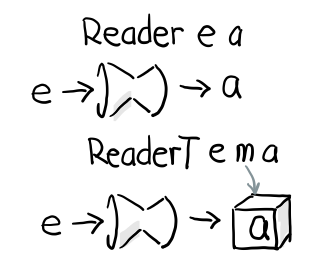
\includegraphics[width=.9\linewidth]{images/p3-ReaderT.png}
\end{center}

\lstset{language=haskell,label= ,caption= ,captionpos=b,numbers=none}
\begin{lstlisting}
instance (Monad m) => Monad (ReaderT e m) where
    return   = lift . return
    r >>= k  = ReaderT $ \ e -> do
        a <- runReaderT r e
        runReaderT (k a) e
\end{lstlisting}

再看看 monad 的实现, 也是一样的, 先 run 一下 \texttt{r e} 得到结果 \texttt{a}, 应用函数 \texttt{k} 到 \texttt{a}, 再 run 一把.


问题是, 这里的 \texttt{return} 里面的 \texttt{lift} 是哪来的?

\lstset{language=haskell,label= ,caption= ,captionpos=b,numbers=none}
\begin{lstlisting}
instance MonadTrans (ReaderT e) where
  lift m = ReaderT (const m)
\end{lstlisting}

\begin{center}
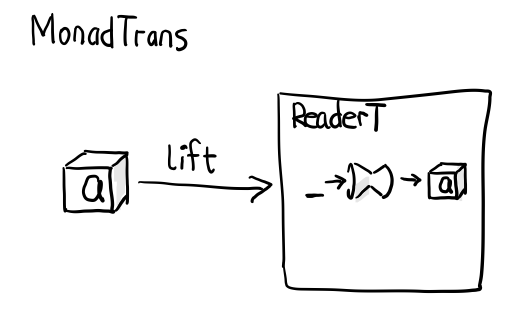
\includegraphics[width=.9\linewidth]{images/p3-MonadTrans-ReaderT-e-m.png}
\end{center}

这个函数 \texttt{lift} 被定义在 MonadTrans 的实例中, 简单的把 m 放到 ReaderT 结果中.

例如, \texttt{lift (Just 1)} 会得到 ReaderT, 其中 e 随意, m 为 Maybe Num

重点需要体会的是, Reader 可以越过 Maybe 直接操作到 Num, 完了再包回来.

有了 ReaderT, 搭配 Id Monad 就很容易创建出来 Reader Monad

\lstset{language=haskell,label= ,caption= ,captionpos=b,numbers=none}
\begin{lstlisting}
type Reader r a= ReaderT r Identity a
\end{lstlisting}

越过 Id read 到 Id 内部, 完了再用 Id 包回来, 不就是 Reader 了么

\lstset{language=haskell,label= ,caption= ,captionpos=b,numbers=none}
\begin{lstlisting}
ReaderT { runReaderT :: r -> Identity a }
-- Identity a is a
ReaderT { runReaderT :: r -> a }
\end{lstlisting}

\chapter{Alternative}
\label{sec:org4cd6769}

这个 typeclass 提供 \texttt{<|>} 函数, 表示要么计算左边, 要么计算右边

\lstset{language=haskell,label= ,caption= ,captionpos=b,numbers=none}
\begin{lstlisting}
class Applicative f => Alternative f where
    empty :: f a
    (<|>) :: f a -> f a -> f a
\end{lstlisting}

\begin{center}
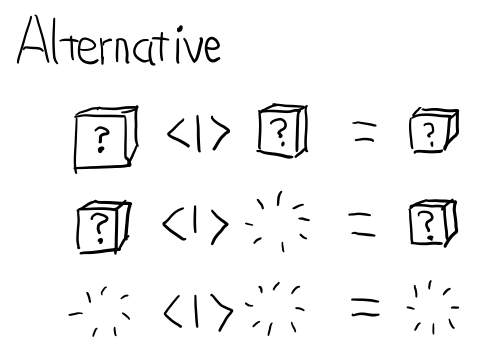
\includegraphics[width=.9\linewidth]{images/p3-Alternative.png}
\end{center}

其实就是 Applicative 的 \texttt{或}

比如:
\lstset{language=haskell,label= ,caption= ,captionpos=b,numbers=none}
\begin{lstlisting}
Just 1 <|> Just 2 -- Just 1
Just 1 <|> Nothing -- Just 1
Nothing <|> Just 1 -- Just 1
Nothing <|> Nothing -- Nothing
\end{lstlisting}

\chapter{MonadPlus}
\label{sec:orgfe8531f}
这跟 Alternative 是一毛一样的, 只是限制的更细, 必须是 Monad才行

\lstset{language=haskell,label= ,caption= ,captionpos=b,numbers=none}
\begin{lstlisting}
class (Alternative m, Monad m) => MonadPlus m where
   mzero :: m a
   mzero = empty
   mplus :: m a -> m a -> m a
   mplus = (<|>)
\end{lstlisting}

看, 实现中直接就调用了 Alternative 的 \texttt{empty} 和 \texttt{<|>}

\chapter{ST Monad}
\label{sec:org9161e44}
ST Monad 跟 State Monad 的功能有些像, 不过更厉害的是, 他不是 immutable 的, 而是 "immutable" 的在原地做修改. 改完之后 runST 又然他回到了 immutable 的 Haskell 世界.

\lstset{language=haskell,label= ,caption= ,captionpos=b,numbers=none}
\begin{lstlisting}
sumST :: Num a => [a] -> a
sumST xs = runST $ do           -- do 后面的事情会是不错的内存操作, runST 可以把它拉会纯的世界
    n <- newSTRef 0             -- 在内存中创建一块并指到 STRef
    forM_ xs $ \x -> do         -- 这跟命令式的for循环改写变量是一毛一样的
        modifySTRef n (+x)
    readSTRef n                 -- 返回改完之后的 n 的值
\end{lstlisting}

\chapter{Free Monad}
\label{sec:orgf40b2be}
上一章说过的 RWS Monad 毕竟是固定搭配,当你的业务需要更多的 Monad 来表示 Effect 时,
我们就需要有那么个小猪手帮我们定义自己的 Monad。

那就是 Free, Free 可以将任意 datatype lift 成为 Monad

\section{Free}
\label{sec:orged5e29d}
先看 Free 什么定义:

\lstset{language=haskell,label= ,caption= ,captionpos=b,numbers=none}
\begin{lstlisting}
data Free f a = Roll (f (Free f a)) | Return a
\end{lstlisting}

其中 \texttt{f} 就是你业务需要的 effect 类型, \texttt{a} 是这个 effect 所产生的返回值类型。

右边两种构造函数,如果把 \texttt{Role} 改成 \texttt{Cons}, \texttt{Return} 改成 \texttt{Nil} 的话, 是不是跟 List 其实是 同构/isomophic 的呢? 所以如果想象成 List, 那么 \texttt{f} 在这里就相当于 List 中的一个元素.

到那时, \texttt{>>=} 的操作又跟 List 略有不同, 我们都知道 \texttt{>>=} 会把每一个元素 map 成 List, 然后 flatten, 但 Free 其实是用来构建
顺序的 effect 的, 所以:

\lstset{language=haskell,label= ,caption= ,captionpos=b,numbers=none}
\begin{lstlisting}
instance Functor f => Monad (Free f) where
  return a        = Return a
  Return a >>= fn = fn a
  Roll ffa >>= fn = Roll $ fmap (>>= fn) ffa
\end{lstlisting}

你会发现 \texttt{>>=} 会递归的 \texttt{fmap} 到 \texttt{Roll} 上, 直到最后一个 \texttt{Return}.

比如, 如果你有一个 program 有三种副作用 Eff1, Eff2, Eff3

\lstset{language=haskell,label= ,caption= ,captionpos=b,numbers=none}
\begin{lstlisting}
data Eff a = Eff1 a | Eff2 a | Eff3 a
program = do
 a <- liftF $ Eff1 1
 b <- liftF $ Eff2 2
 c <- liftF $ Eff3 3
 return a + b + c
\end{lstlisting}

如果我们把 program 展开, 每一步 \texttt{>>=} 大概是这样:

\lstset{language=haskell,label= ,caption= ,captionpos=b,numbers=none}
\begin{lstlisting}
liftF $ Eff1 1
\end{lstlisting}

展开既是:

\lstset{language=haskell,label= ,caption= ,captionpos=b,numbers=none}
\begin{lstlisting}
Roll (Eff1 (Return 1))
\end{lstlisting}

代入到 program 即:
\lstset{language=haskell,label= ,caption= ,captionpos=b,numbers=none}
\begin{lstlisting}
program = Roll (Eff1 (Return 1)) >>= \a -> do
   b <- liftF $ Eff2 2
   c <- liftF $ Eff3 3
   return a + b + c
\end{lstlisting}

用 Free 的 \texttt{>>=} 公式 \texttt{Roll ffa >>= fn = Roll \$ fmap (>>= fn) ffa} 去展开上面就得到:

\lstset{language=haskell,label= ,caption= ,captionpos=b,numbers=none}
\begin{lstlisting}
program = Roll $ Eff1 (Return 1 >>= fn1)) where
  fn1 = \a -> do
   b <- liftF $ Eff2 2
   c <- liftF $ Eff3 3
   return a + b + c
\end{lstlisting}

\texttt{Return 1 >>= fn1} 我们都知道怎么展开:

\lstset{language=haskell,label= ,caption= ,captionpos=b,numbers=none}
\begin{lstlisting}
program = Roll $ Eff1 (fn1 1) where
  fn1 = \a -> do
   b <- liftF $ Eff2 2
   c <- liftF $ Eff3 3
   return a + b + c
\end{lstlisting}

展开 \texttt{fn1}

\lstset{language=haskell,label= ,caption= ,captionpos=b,numbers=none}
\begin{lstlisting}
program = Roll $ Eff1 do
   b <- liftF $ Eff2 2
   c <- liftF $ Eff3 3
   return 1 + b + c
\end{lstlisting}


同样的步骤展开 Eff2
\lstset{language=haskell,label= ,caption= ,captionpos=b,numbers=none}
\begin{lstlisting}
program = Roll $ Eff1 $ Roll $ Eff2 do
   c <- liftF $ Eff3 3
   return 1 + 2 + c
\end{lstlisting}

和 Eff3

\lstset{language=haskell,label= ,caption= ,captionpos=b,numbers=none}
\begin{lstlisting}
program = Roll $ Eff1 $ Roll $ Eff2 $ Roll $ Eff3 do
   return 1 + 2 + 3
\end{lstlisting}

最后的 program 是不是很像 List 的 Cons 和 Nil 呢?

\lstset{language=haskell,label= ,caption= ,captionpos=b,numbers=none}
\begin{lstlisting}
program = Roll $ Eff1 $ Roll $ Eff2 $ Roll $ Eff3 $ Return 1 + 2 + 3
\end{lstlisting}


但是, 细心的你可能早都发现了 \texttt{Eff} 这货必须是个 \texttt{Functor} 才行. 那我们如何随便定义一个 \texttt{data Eff} 直接能生成 \texttt{Functor Eff} 的实例呢?

\section{Coyoneda}
\label{sec:org496bb2d}

希望你还依然记得第一部分的米田 \sout{共} 引理

\lstset{language=haskell,label= ,caption= ,captionpos=b,numbers=none}
\begin{lstlisting}
data CoYoneda f a = forall b. CoYoneda (b -> a) (f b)
\end{lstlisting}

\begin{center}
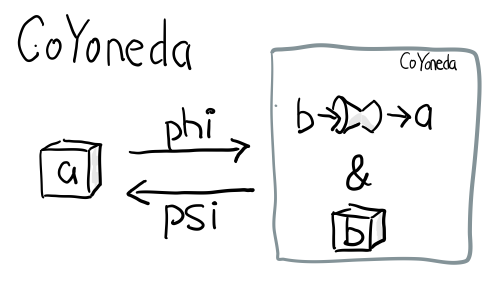
\includegraphics[width=.9\linewidth]{images/p3-CoYoneda.png}
\end{center}

事实上很简单可以把任何 \texttt{f} 变成 \texttt{CoYoneda f}

\lstset{language=haskell,label= ,caption= ,captionpos=b,numbers=none}
\begin{lstlisting}
phi :: f a -> CoYoneda f a
phi fa = CoYoneda id fa
\end{lstlisting}

\begin{center}
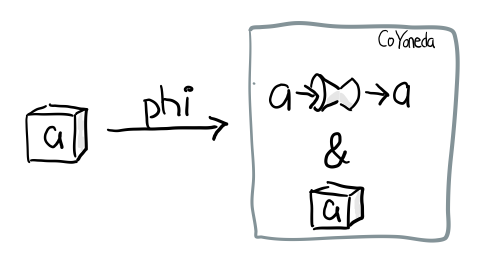
\includegraphics[width=.9\linewidth]{images/p3-CoYoneda-phi.png}
\end{center}

诀窍就是 \texttt{id}, 也就是你把 \texttt{b} 变成 \texttt{a}, 再把 \texttt{fa} 放到 \texttt{CoYoneda} 里就好了

当 \texttt{f} 是 \texttt{Functor} 时, 又可以把 \texttt{CoYoneda} 变成 \texttt{f}

\lstset{language=haskell,label= ,caption= ,captionpos=b,numbers=none}
\begin{lstlisting}
psi :: Functor f => CoYoneda f a -> f a
psi (CoYoneda g fa) = fmap g fa
\end{lstlisting}

\begin{center}
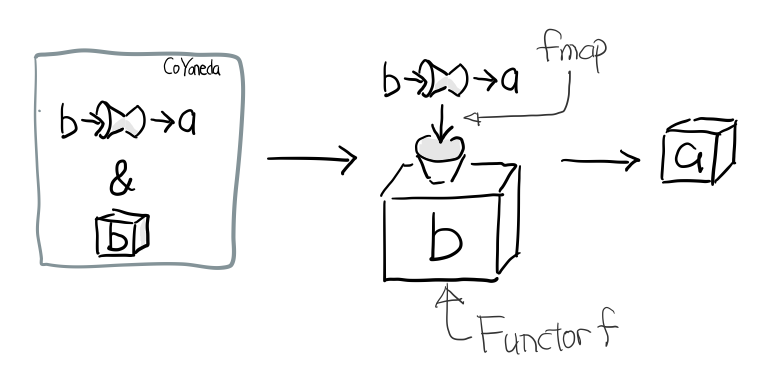
\includegraphics[width=.9\linewidth]{images/p3-CoYoneda-psi.png}
\end{center}

反过来的这个不重要, 重要的是 \texttt{phi}, 因为如果你可以把任何 \texttt{f} 变成 \texttt{CoYoneda f}, 而 \texttt{CoYoneda f} 又是 \texttt{Functor},
我们不就免费得到一个 \texttt{Functor}?

\lstset{language=haskell,label= ,caption= ,captionpos=b,numbers=none}
\begin{lstlisting}
instance Functor (Coyoneda f) where
  fmap f (Coyoneda g fb) = Coyoneda (f . g) fb
\end{lstlisting}

\section{Free Functor}
\label{sec:orged06f0c}
比如我们的 \texttt{Eff} 就可以直接通过 \texttt{phi} 变成 \texttt{CoYoneda Eff}, 从而得到免费的 Functor

\lstset{language=haskell,label= ,caption= ,captionpos=b,numbers=none}
\begin{lstlisting}
data Eff a = Eff1 a | Eff2 a | Eff3 a
program = Roll (phi (Eff1 (Roll (phi (Eff2 (Return Int))))))
\end{lstlisting}

\begin{center}
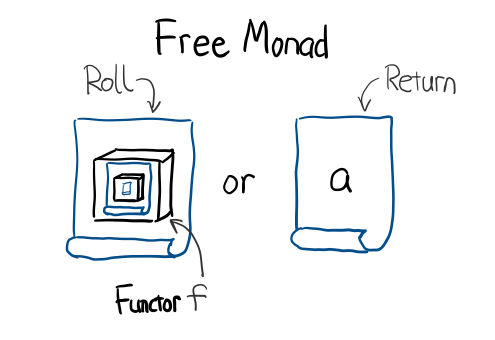
\includegraphics[width=.9\linewidth]{images/p3-Free.png}
\end{center}

\section{Interpreter}
\label{sec:org66a58c8}
构造完一个 free program 后,我们得到的是一个嵌套的数据结构, 当我们需要 run 这个 program 时, 我们需要 foldMap 一个
Interpreter 去一层层拨开 这个 free program.

\lstset{language=haskell,label= ,caption= ,captionpos=b,numbers=none}
\begin{lstlisting}
foldMap :: Monad m => (forall x . f x -> m x) -> Free f a -> m a
foldMap _ (Return a)  = return a
foldMap f (Roll a) = f a >>= foldMap f
\end{lstlisting}

\chapter{Free Monoid}
\label{sec:orga863419}
\chapter{Eff}
\label{sec:orgef082b8}

\chapter{Comonad}
\label{sec:org058f2f5}
\end{document}
